%%%%% SOME OPTIONS %%%%% 
\newcommand{\german}{true} % germanTrue or false --> Switch between german and english headers / titlepage
\newcommand{\coloredTitlePage}{true} % Switch between colored and BW titlepage
\newcommand{\company}{false}
\newcommand{\ECE}{true}
%%%%% Required Settings for the template %%%%%
%%%%% Configuration Package for the ThesisTemplate ECE / AEE %%%%%%
%
% Created by Mayer Florian October/2016
% v1.0

%======= DocumentClass ===========%
\documentclass[11pt, openright]{book} %Extarticle supports more FontSizes

%========= ADD Latex PACKAGES =========%
\usepackage{tabularx}         
\usepackage{parskip}%NEW
\newcolumntype{x}[1]{!{\centering\arraybackslash\vrule width #1}}
\usepackage{booktabs}
\usepackage[utf8]{inputenc} %to allow vowel mutations
\usepackage{tikz} % Schematic creator with TikZ in LaTex
\usepackage{geometry,titlesec,layout}
\usepackage{subfigure}
\usepackage{xcolor,colortbl}
%\usepackage{graphicx,rotating}
\usepackage{float}
\usepackage{epstopdf}
\usepackage[titles]{tocloft}
\usepackage{blindtext}
\usepackage{anyfontsize}
\usepackage{setspace,varwidth}
\usepackage{ifthen}
\usepackage{multicol,multirow}
\usepackage{makecell}
\usepackage[stable,bottom,hang,splitrule,multiple]{footmisc}% customize footnotes
\usepackage[final]{listings}% program code listings
\usepackage[%
headtopline,plainheadtopline,% activate all lines (header and footer)
headsepline,plainheadsepline,%
footsepline,plainfootsepline,%
footbotline,plainfootbotline,%
nouppercase% auto update \..mark
]{scrpage2}% (KOMA)

\usepackage[%
breaklinks=true,% allow line break in links
colorlinks=true,% if false: framed link
linkcolor=black,anchorcolor=black,citecolor=black,filecolor=black,%
menucolor=black,urlcolor=black]{hyperref}% hyperlinks for references

\usepackage{amssymb}
\usepackage{emptypage}
\usepackage{glossaries}
\usepackage{appendix}
\usepackage{mdframed}
\usepackage{etoolbox}
\usepackage{chngcntr} 

\usepackage{textcomp}
\usepackage{lmodern}
\usepackage[european, straightvoltages, americaninductors]{circuitikz}

%========= ADD TikZ PACKAGES =========%
\usetikzlibrary{matrix,calc,positioning,arrows,shapes}
\usetikzlibrary{decorations.pathreplacing}

%======= END ADD PACKAGES =======%
\geometry{a4paper,twoside,%
	%textheight=205mm, %246mm,%
	textwidth=160mm,%
	top = 3cm,
	bottom = 4.5cm,
	heightrounded=false,% round textheight to multiple of lines (avoids overfull vboxes)
	ignoreall=true,% do not include header, footer, and margins in calculations
	marginparsep=5pt,% marginpar only used for signs (centered), thus only small sep. needed
	marginparwidth=10mm,% prevent margin notes to be out of page
	hmarginratio=1:2,
	voffset = 2.25mm,
	%headheight = 16mm,
	headsep = 9mm,
	footskip = 13mm
}
\linespread{1.4}
%======= DEFINE COLORS ===========%
\definecolor{DENcol}{RGB}{35,171,196} % Department Colour


%======= Re-Define Essential Commands and store old ones ======%
\newcommand{\ChapterFont}{qag}
\newcommand{\WorkingFont}{\rmdefault}
\renewcommand{\familydefault}{\WorkingFont}
\normalfont

%======= Set Depths of TOC / TOF / TOL =======%

\renewcommand{\cftchapfont}{\bf\large\fontfamily{\sfdefault}\selectfont}
\renewcommand{\cftpartfont}{\bf\large\fontfamily{\sfdefault}\selectfont}

\ifthenelse{\equal{\german}{true}}
{
\usepackage[ngerman]{babel}
\renewcommand{\lstlistingname}{Programmcode} 
}
%====== Usefull Additional Commands =======%

% Make clickable footnote
    \newcommand{\hyperfootnote}[1][]{\def\ArgI\hyperfootnoteRelay}
    % relay to new command to make extra optional command possible
    \newcommand\hyperfootnoteRelay[2][]{\href{#1#2}{\ArgI}\footnote{\href{#1#2}{#2}}}
    % the first optional argument is now in \ArgI, the second is in #1
    %http://www.brechtdeman.com/blog/latex-clickable-footnote.html
    % Simple (no arguments)
    %    \hyperfootnote{http://www.mywebsite.com}
    % Link text (1 argument)
    %   \hyperfootnote[My website]{http://www.mywebsite.com}
    % Link text and invisible prefix (2 arguments)
    %   \hyperfootnote[My website][http://]{www.mywebsite.com}

\newcommand{\ie}{i.\,e.}
\newcommand{\Ie}{I.\,e.}
\newcommand{\eg}{e.\,g.}
\newcommand{\Eg}{E.\,g.} 

%====== Heading Commands =======%

\pagestyle{scrheadings}%
% \setlength\parindent{0cm}% no indentation for first line of new paragraph
% \raggedbottom% do not try to fill pages

% header and footer size
\setheadwidth{text}% set header width to textwidth
\setfootwidth{text}% set footer width to textwidth
\setheadtopline[textwithmarginpar]{0.25pt}% set up separator lines (greater width than text)
\setheadsepline[textwithmarginpar]{0.25pt}
\setfootsepline[textwithmarginpar]{0.25pt}
\setfootbotline[textwithmarginpar]{0.25pt}

\renewcommand*\chaptermark[1]{\markleft{\thechapter~#1}}
\renewcommand*\sectionmark[1]{\markright{\thesection~#1}} 

\clearscrheadfoot % clear everything
\ihead[]{}%
\ohead[\ShortTitle]{\footnotesize\headmark}%
%\cfoot[\footnotesize\ConfidNote]{\footnotesize\ConfidNote}%

\ofoot[\ifthenelse{\equal{\thepage}{}}{\pagemark}{--~~\pagemark~~--}]{\ifthenelse{\equal{\thepage}{}}{\pagemark}{--~~\pagemark~~--}}%

%============== Chapter / Section / Subsection Style ==== %
\titleformat{\part}[display]
   {\fontfamily{\sfdefault}\bfseries\fontsize{26}{26}\selectfont\filcenter}
   {\fontfamily{\sfdefault}\bfseries\fontsize{30}{22}\selectfont\partname{} \thepart}
   {0.5em}
   {}

\titleformat{\chapter}[display]
{\fontfamily{\sfdefault}\bfseries\fontsize{22}{22}\selectfont}%\
{
\begin{tikzpicture}[overlay]
	\node (CoolTitle) at (12,1) [opacity=0.325]{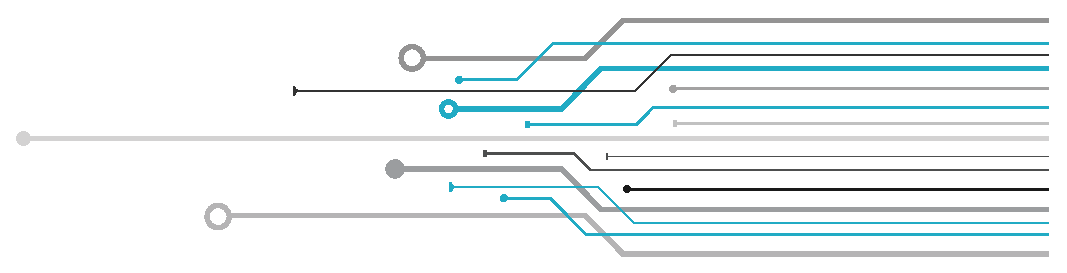
\includegraphics[scale=0.75]{temp_graphics/chapterBacking.eps}};
	\node (titleNumber) at ($(CoolTitle)+(3,0)$) {\textcolor{black!80}{\fontfamily{\ChapterFont}\bfseries\Large\fontsize{80}{80}\selectfont\thechapter}};
\end{tikzpicture}
}
{0.05em}%
{\vspace{0.25ex}\filleft}%

\titleformat{\section}{\Large \bfseries \sffamily}{\thesection}{1 em}{}
\titleformat{\subsection}{\large \bf \sffamily}{\thesubsection}{1 em}{}
\titleformat{\subsubsection}{\large \bf \sffamily}{\thesubsubsection}{1 em}{}

%%%% CLEAR DOUBLE-PAGE
% redefine cleardoublepage...
\makeatletter
\renewcommand{\cleardoublepage}{\clearpage\if@twoside\ifodd\c@page\else\thispagestyle{plain}\hbox{}\newpage\if@twocolumn\hbox{}\newpage\fi\fi\fi}
% ...and define empty double page (e.g., for title sheet)
\newcommand{\emptydoublepage}{\clearpage\if@twoside\ifodd\c@page\else\thispagestyle{empty}\hbox{}\newpage\if@twocolumn\hbox{}\newpage\fi\fi\fi}%
% ...and also an empty single page
\newcommand{\emptypage}{\clearpage\thispagestyle{empty}\hbox{}\newpage\if@twocolumn\hbox{}\newpage\fi}%
\makeatother

%%%%% Correct Even and Odd Pages %%%%%
\let\tmp\oddsidemargin
\let\oddsidemargin\evensidemargin
\let\evensidemargin\tmp
\reversemarginpar

% code listings
\lstloadlanguages{Bash,VHDL,Matlab,[ANSI]C,Java,[LaTeX]TeX}

\lstset{
	frame=top,frame=bottom,
	basicstyle=\fontsize{8}{8}\normalfont\sffamily,    % the size of the fonts that are used for the code
	stepnumber=1,                           % the step between two line-numbers. If it is 1 each line will be numbered
	numbersep=6pt,                         % how far the line-numbers are from the code
	tabsize=2,                              % tab size in blank spaces
	extendedchars=true,                     %
	breaklines=true,                        % sets automatic line breaking
	captionpos=t,                           % sets the caption-position to top
	mathescape=true,
	stringstyle=\color{black}\ttfamily, % Farbe der String
	showspaces=false,           % Leerzeichen anzeigen ?
	showtabs=false,             % Tabs anzeigen ?
	xleftmargin=15pt,
	framexleftmargin=14pt,
	framexrightmargin=9pt,
	framexbottommargin=5pt,
	framextopmargin=5pt,
	showstringspaces=false,      % Leerzeichen in Strings anzeigen ?
	numbers = left,
	linewidth = 150mm
}
%%%% MDBOX Setup
\mdfsetup{%
middlelinecolor=red,
middlelinewidth=2pt,
backgroundcolor=DENcol!10,
roundcorner=10pt,
topline = false,
bottomline = false,
rightline = false,
linecolor = DENcol,
linewidth = 10pt}

%%%% GET RID OF OVERFULL BOXING WARNINGS %%%%
%\overfullrule=5pt
\setlength{\headheight}{1.1\baselineskip}
\raggedbottom

%%%%%%%%%%%%%
\counterwithout{footnote}{chapter}


\usepackage{hyperref}

\makeglossaries

\makeatletter
\ctikzset{current arrow color/.initial=black}% create key

\let\old@circ@drawcurrent=\pgf@circ@drawcurrent
\def\pgf@circ@drawcurrent{\old@circ@drawcurrent}

\pgfdeclareshape{currarrow}{
\anchor{center}{
\pgfpointorigin
}
\anchor{tip}{
\pgfpointorigin
    \pgf@circ@res@step = \pgf@circ@Rlen
        \divide \pgf@circ@res@step by 16
\pgf@x  =\pgf@circ@res@step
}
\behindforegroundpath{      

\pgfscope
    \pgf@circ@res@step = \pgf@circ@Rlen
    \divide \pgf@circ@res@step by 16

    \pgfpathmoveto{\pgfpoint{-.7\pgf@circ@res@step}{0pt}}
    \pgfpathlineto{\pgfpoint{-.7\pgf@circ@res@step}{-.8\pgf@circ@res@step}}
    \pgfpathlineto{\pgfpoint{1\pgf@circ@res@step}{0pt}}
    \pgfpathlineto{\pgfpoint{-.7\pgf@circ@res@step}{.8\pgf@circ@res@step}}
    \pgfpathlineto{\pgfpoint{-.7\pgf@circ@res@step}{0pt}}           
    \pgfsetcolor{\pgfkeysvalueof{/tikz/circuitikz/current arrow color}}
    \pgfusepath{draw,fill}

\endpgfscope
}
}
\pgfdeclareshape{flowarrow}{
    \anchor{center}{\pgfpointorigin}
    \anchor{tip}{
    \pgfpointorigin
        \pgf@circ@res@step = \pgf@circ@Rlen
            \divide \pgf@circ@res@step by 16
    \pgf@x  =\pgf@circ@res@step
    }
\behindforegroundpath{
    \pgfscope
        \pgf@circ@res@step = \pgf@circ@Rlen
        \divide \pgf@circ@res@step by 4
        \pgfpathmoveto{\pgfpoint{-\pgf@circ@res@step}{0pt}}
        \pgfpathlineto{\pgfpoint{\pgf@circ@res@step}{0pt}}
        %\pgfsetcolor{\pgfkeysvalueof{/tikz/circuitikz/color}}
  \pgfsetcolor{\pgfkeysvalueof{/tikz/circuitikz/current arrow color}}
        \pgfusepath{draw}
        \pgftransformshift{\pgfpoint{\pgf@circ@res@step}{0pt}}
        \pgfnode{currarrow}{tip}{}{}{\pgfusepath{fill}}
    \endpgfscope
}
}

\makeatletter
\newcommand{\myscope}[2] % #1 = name , #2 = rotation angle
{\draw[thick,rotate=#2] (#1) circle (12pt)
 (#1) ++(-0.35,-0.1) -- ++(0.3,0.3) --++(0,-0.3)-- ++(0.3,0.3) --++(0,-0.3);
}

\begin{document}
%%%%% ThesisTemplate ECE / AEE %%%%%%
%
% Created by Mayer Florian October/2016
% v1.0

%============== Glossary Command ==== %

\newglossaryentry{SCSS}{name=SCSS, description={Single Channel Source Separation}} 
\newglossaryentry{ITD}{name=ITD, description={Interaural Time Difference}}
\newglossaryentry{PASCSS}{name=PASCSS, description={Phase-Aware Single Channel Source Separation}}
\newglossaryentry{CASA}{name=CASA, description={Computational Auditory Scene Analysis}}
\newglossaryentry{NMF}{name=NMF, description={Non-Negative Matrix Factorization}}
\newglossaryentry{CMF}{name=CMF, description={Complex Matrix Factorization}}
\newglossaryentry{STFT}{name=STFT, description={Short-Time Fourier Transformation}}
\newglossaryentry{DTFT}{name=DTFT, description={Discrete-Time Fourier Transformation}}
\newglossaryentry{ISTFT}{name=ISTFT, description={Inverse Short-Time Fourier Transformation}}
\newglossaryentry{IBM}{name=IBM, description={Ideal Binary Mask}}
\newglossaryentry{IRM}{name=IRM, description={Ideal Ratio Mask}}
\newglossaryentry{SNR}{name=SNR, description={Signal-to-Noise Ratio}}
\newglossaryentry{DNN}{name=DNN, description={Deep neural network}}
\newglossaryentry{SVM}{name=SVM, description={Support vector machine}}
\newglossaryentry{KL-divergence}{name=KL-divergence, description={Kullback-Leibler divergence}}
\newglossaryentry{MPE}{name=MPE, description={Multipitch Estimator}} 
\newglossaryentry{PEFAC}{name=PEFAC, description={Pitch Estimation Filter with Amplitude Compression}}  
\newglossaryentry{GMM}{name=GMM, description={Gaussian mixture models}} 
\newglossaryentry{GLA}{name=GLA, description={Griffin and Lim Algorithm}}  
\newglossaryentry{MISI}{name=MISI, description={Multiple Input Spectrogram Inversion}}
\newglossaryentry{PPR}{name=PPR, description={Partial Phase Reconstruction}}
\newglossaryentry{ISSIR}{name=ISSIR, description={Partial Phase Reconstruction for Informed Source Separation}}
\newglossaryentry{FHMM}{name=FHMM, description={Factorial Hidden Markov Models}}
\newglossaryentry{HMM}{name=HMM, description={Hidden Markov Models}}
\newglossaryentry{SHR}{name=SHR, description={Subharmonic to harmonic ratio}}
\newglossaryentry{POC}{name=POC, description={Proof of Concept}}
\newglossaryentry{SSR}{name=SSR, description={Signal-to-Signal Ratio}}
\newglossaryentry{GPE}{name=GPE, description={Gross-Pitch Error}}
\newglossaryentry{MMSE}{name=MMSE, description={Minimum Mean Squared Error}}
\newglossaryentry{PESQ}{name=PESQ, description={Perceptual Evaluation of Speech Quality}}
\newglossaryentry{STOI}{name=STOI, description={Short-time objective intelligibility}}
\newglossaryentry{BSS-Eval}{name=BSS-Eval, description={Blind Source separation evaluation}}
\newglossaryentry{SDR}{name=SDR, description={Signal-to-Distortion Ratio}}
\newglossaryentry{SIR}{name=SIR, description={Signal-to-Interference Ratio}}
\newglossaryentry{SAR}{name=SAR, description={Signal-to-Artifact Ratio}}
\newglossaryentry{PE}{name=PE, description={Phase Estimation}}
\newglossaryentry{SSN}{name=SSN, description={Speech-Shaped Noise}}
%frontmatter inluding:
%titlepage, abstract, acknowledgments, declaration, toc, lof, lot
\frontmatter
\renewcommand{\thepage}{\Roman{page}}

% titlepage ----> changelog
%% Author: Mayer Florian (ECE)
%%
%% 10.10.16 ---------> Created TitlePage 

\renewcommand{\familydefault}{\sfdefault}
\normalfont 

%%%%% Now we add YOUR Personal DATA %%%%%
%%%%% What you enter here, will be written to the variables used within this document !! %%%%%%
\ifthenelse{\equal{\german}{true}}
{
	\newcommand{\ThesisTitle}{Analoge Signalverarbeitung}
	\newcommand{\ThesisSubtitle}{Laborprotokoll}
	\newcommand{\ShortTitle}{ASV Laborprotokoll} % needed for headers within your document 
	\newcommand{\ThesisAuthor}{Anderle Fabian, Grebien Alexander}
	\newcommand{\ThesisDate}{Graz, SS2020}
	\newcommand{\ThesisType}{} % Bachelor Thesis
	%\newcommand{\Organization}{am Bachelor Studiengang Elektronik und Computer Engineering \\ der FH JOANNEUM -- University of Applied Sciences, Austria}
	\newcommand{\Supervisor}{} % Supervisor 1 \\ Supervisor 2 \\ ...
	\newcommand{\CoSupervisor}{} % Supervisor 1 \\ Supervisor 2 \\ ...
	\newcommand{\Assessors}{}
	\newcommand{\SpecialNote}{}
	%%%%%%%%%%%%%%%%%%%%%%%%%%%%%%%%
}
{
	\newcommand{\ThesisTitle}{Title of your Thesis}
	\newcommand{\ThesisSubtitle}{Additional Title}
	\newcommand{\ShortTitle}{Short Title} % needed for headers within your document 
	\newcommand{\ThesisAuthor}{Author}
	\newcommand{\ThesisDate}{Graz, \today}
	\newcommand{\ThesisType}{Bachelor thesis 1 / 2} % Bachelor Thesis
	%\newcommand{\Organization}{am Bachelor Studiengang Elektronik und Computer Engineering \\ der FH JOANNEUM -- University of Applied Sciences, Austria}
	\newcommand{\Supervisor}{Your Supervisor} % Supervisor 1 \\ Supervisor 2 \\ ...
	\newcommand{\CoSupervisor}{Your External-Supervisor} % Supervisor 1 \\ Supervisor 2 \\ ...
	\newcommand{\Assessors}{Prüfer Eins \\ Prüfer Zwei \\ weitere....}
	\newcommand{\SpecialNote}{}
}
%%%%%%%%%%%%%%%%%%%%%%%%%%%%%%%%

\ifthenelse{\equal{\coloredTitlePage}{true}}
{
\newcommand{\bcol}{DENcol}
\newcommand{\tcol}{white}
}{
\newcommand{\bcol}{white}
\newcommand{\tcol}{black}
}

\thispagestyle{empty}

%====== Create Sizes For Title what so ever ====== %
\newcommand{\MainTitlesize}{\bf\fontsize{24}{24}\selectfont}
\newcommand{\SubTitlesize}{\bf\fontsize{16}{16}\selectfont}
\newcommand{\Namesize}{\bf\fontsize{14}{14}\selectfont}

\ifthenelse{\equal{\german}{true}}
{
\begin{tikzpicture}[overlay]

\ifthenelse{\equal{\company}{true}}
{
	\ifthenelse{\equal{\ECE}{true}}
	{
		\node (Logo) at (9cm,-1) [anchor = east] {
\includegraphics[scale = 1]{temp_graphics/company_logo.eps}};
		\node (Logo2) at (17cm,-0.9) [anchor = east] {
\includegraphics[scale = 1.1]{temp_graphics/logo_FHJ_ECE_white.eps}};
	}
	{
		\node (Logo) at (9cm,-1) [anchor = east] {
\includegraphics[scale = 1]{temp_graphics/company_logo.eps}};
		\node (Logo2) at (17cm,-0.9) [anchor = east] {
\includegraphics[scale = 1.1]{temp_graphics/ecm_logo_eps.eps}};
	}
}
{
	\ifthenelse{\equal{\ECE}{true}}
	{
		\node (Logo) at (17cm,-0.9) [anchor = east] {
\includegraphics[scale = 1.1]{temp_graphics/logo_FHJ_ECE_white.eps}};
	}
	{
		\node (Logo) at (16cm,-0.9) [anchor = east] {
\includegraphics[scale = 0.9]{temp_graphics/ecm_logo_eps.eps}};
	}
}

%% ===== CREATE background ===== %%
% Background Box
\node (boxOne)  at (7cm,-12) [minimum width=1.1\paperwidth,fill = \bcol, minimum height=18cm, inner sep=0pt] {};

\node (ThesisTitle) [color = \tcol, font = \MainTitlesize, align = flush right, anchor = north east] at (16,-4){\ThesisTitle};

\node (ThesisSubtitle) [color = \tcol, font = \SubTitlesize, align = flush right, anchor = north east] at ($(ThesisTitle.south east) + (0,-0.25em)$){\ThesisSubtitle};

\node (ThesisType) [color = \tcol, font = \SubTitlesize, align = flush right, anchor = north east] at ($(ThesisSubtitle.south east) + (0,-3em)$){\ThesisType};

\node (AuthName) [color = \tcol, font = \large, align = flush right, anchor = north east] at ($(ThesisType.south east) + (0,-2em)$){\bf{angefertigt von:} \\ \ThesisAuthor};



\ifthenelse{\equal{\ECE}{true}}
{
	\node (Organization) [color = \tcol, font = \large, align = flush right, anchor = north east] at ($(AuthName.south east) + (0,-3em)$){am Bachelor-Studiengang Elektronik und Computer Engineering \\ der FH JOANNEUM -- University of Applied Sciences, Austria};
}
{
	\node (Organization) [color = \tcol, font = \large, align = flush right, anchor = north east] at ($(AuthName.south east) + (0,-3em)$){am Master-Studiengang Electronics and Computer Engineering \\ der FH JOANNEUM -- University of Applied Sciences, Austria};
}

\node (Supervisor) [color = \tcol, font = \large, align = flush right, anchor = north east] at ($(Organization.south east) + (0,-3em)$){\bf{ } \\ \Supervisor};

\ifthenelse{\equal{\company}{true}}
{
	\node (COSupervisor) [color = \tcol, font = \large, align = flush right, anchor = north east] at ($(Supervisor.south east) + (0,-3em)$){\bf{extern Betreut von:} \\ \CoSupervisor};
	
	\node (ThesisDate) [color = \tcol, font = \large, align = flush right, anchor = north east] at ($(COSupervisor.south east) + (0,-3em)$){\bf\ThesisDate};
}
{

\node (ThesisDate) [color = \tcol, font = \large, align = flush right, anchor = north east] at ($(Supervisor.south east) + (0,-3em)$){\bf\ThesisDate};

}

\node (SpecialNote) [color = \tcol, font = \large, align = center, anchor = north east] at ($(ThesisDate.south east) + (0,-3em)$){\begin{varwidth}{14cm} \SpecialNote \end{varwidth}};

\end{tikzpicture}	
}
{
\begin{tikzpicture}[overlay]

\ifthenelse{\equal{\company}{true}}
{
	\ifthenelse{\equal{\ECE}{true}}
	{
		\node (Logo) at (9cm,-1) [anchor = east] {
\includegraphics[scale = 1]{temp_graphics/company_logo.eps}};
		\node (Logo2) at (17cm,-0.9) [anchor = east] {
\includegraphics[scale = 1.1]{temp_graphics/logo_FHJ_ECE_white.eps}};
	}
	{
		\node (Logo) at (9cm,-1) [anchor = east] {
\includegraphics[scale = 1]{temp_graphics/company_logo.eps}};
		\node (Logo2) at (17cm,-0.9) [anchor = east] {
\includegraphics[scale = 1.1]{temp_graphics/ecm_logo_eps.eps}};
	}
}
{
	\ifthenelse{\equal{\ECE}{true}}
	{
		\node (Logo) at (17cm,-0.9) [anchor = east] {
\includegraphics[scale = 1.1]{temp_graphics/logo_FHJ_ECE_white.eps}};
	}
	{
		\node (Logo) at (16cm,-0.9) [anchor = east] {
\includegraphics[scale = 0.9]{temp_graphics/ecm_logo_eps.eps}};
	}
}

%% ===== CREATE background ===== %%
% Background Box
\node (boxOne)  at (7cm,-12) [minimum width=1.1\paperwidth,fill = \bcol, minimum height=18cm, inner sep=0pt] {};

\node (ThesisTitle) [color = \tcol, font = \MainTitlesize, align = flush right, anchor = north east] at (16,-4){\ThesisTitle};

\node (ThesisSubtitle) [color = \tcol, font = \SubTitlesize, align = flush right, anchor = north east] at ($(ThesisTitle.south east) + (0,-0.25em)$){\ThesisSubtitle};

\node (ThesisType) [color = \tcol, font = \SubTitlesize, align = flush right, anchor = north east] at ($(ThesisSubtitle.south east) + (0,-3em)$){\ThesisType};

\node (AuthName) [color = \tcol, font = \large, align = flush right, anchor = north east] at ($(ThesisType.south east) + (0,-2em)$){\bf{created by:} \\ \ThesisAuthor};

\ifthenelse{\equal{\ECE}{true}}
{
	\node (Organization) [color = \tcol, font = \large, align = flush right, anchor = north east] at ($(AuthName.south east) + (0,-3em)$){at the bachelor degree programme Elektronik und Computer Engineering \\ of FH JOANNEUM -- University of Applied Sciences, Austria};
}
{
	\node (Organization) [color = \tcol, font = \large, align = flush right, anchor = north east] at ($(AuthName.south east) + (0,-3em)$){at the masters degree programme Elektronics and Computer Engineering \\ of FH JOANNEUM -- University of Applied Sciences, Austria};	
}

\node (Supervisor) [color = \tcol, font = \large, align = flush right, anchor = north east] at ($(Organization.south east) + (0,-3em)$){\bf{supervised by:} \\ \Supervisor};

\ifthenelse{\equal{\company}{true}}
{
	\node (COSupervisor) [color = \tcol, font = \large, align = flush right, anchor = north east] at ($(Supervisor.south east) + (0,-3em)$){\bf{external supervisor:} \\ \CoSupervisor};
	
	\node (ThesisDate) [color = \tcol, font = \large, align = flush right, anchor = north east] at ($(COSupervisor.south east) + (0,-3em)$){\bf\ThesisDate};
}
{
	\node (ThesisDate) [color = \tcol, font = \large, align = flush right, anchor = north east] at ($(Supervisor.south east) + (0,-3em)$){\bf\ThesisDate};
}

%\node (Assessor) [color = \tcol, font = \large, align = flush right, anchor = north east] at ($(Supervisor.south east) + (0,-3em)$){\bf{Prüfer:} \\ \Assessors};

\node (SpecialNote) [color = \tcol, font = \large, align = center, anchor = north east] at ($(ThesisDate.south east) + (0,-3em)$){\begin{varwidth}{14cm} \SpecialNote \end{varwidth}};

\end{tikzpicture}	
}
\renewcommand{\familydefault}{\WorkingFont}
\normalfont


\tableofcontents
\printglossary
%mainmatter inluding: Parts, chapters, sections, appendicies
\mainmatter
%Hier die verschiedenn tex_Dokumente der Labore einfügen
\chapter{Operationsverstärker Grundschaltungen}
\section{Spannungsfolger mit uA741}
\subsection{Aufgabenstellung}
Die Offsetspannung des Operationsverstärkers ist mit dem Tischmultimeter zu messen, dabei ist mittels eines Potentiometers ein Offsetabgleich vorzunehmen. Danach soll das Gehäuse mit Kältespray abgekühlt werden und die damit verschobene Offsetverschiebung aufzunehmen. 

Die Grenzfrequenz dieser Schaltung ist zu bestimmen und mit einer PSPICE Simulation zu vergleichen. Dabei sollte eine Eingangsspannung mit $V_{PP} = 100 \rm mV$ verwendet werden. 

Der Aussteuerbereich bei einer Eingangsfrequenz von $f=1 \rm kHz$ ist zu bestimmen, dabei sind die Messungen sowohl mit eine Last von $R_{Last} = 2 \rm k\Omega$ als auch ohne Last vorzunehmen. Dafür ist die Amplitude der Eingangsspannung schrittweise zu erhöhen bis eine deutliche Übersteuerung in beiden Halbwellen zu sehen ist. Für diesen Zweck ist die Versorgungsspannung auf $V_{CC} = 10\rm V$ und $V_{EE} = -10 \rm V$ zu verringern. 

Danach ist die negative Versorgungsspannung auf $V_{EE} = -5V$ zu verringern und das daraus resultierende Verhalten zu dokumentieren.

Durch anlegen einer Rechteckspannung ist die Slew Rate des Verstärkers zu bestimmen. Diese ist sowohl mit einem Lastwiderstand von $R_{Last} = 2\rm k\Omega$, als auch mit einer kapazitiven Last von $C_{Last} = 100 \rm nF$ zu bestimmen. 

Durch Kenntnis der maximalen Slew Rate ist nun die sinusförmige Spannung am Eingang anzulegen, welche gerade noch unverzerrt übertragen werden kann. Ausgehend von dieser Spannung ist nun die Frequenz schrittweise zu erhöhen bis eine deutliche Verzerrung zu erkennen ist. 
\begin{figure}[H]
    \centering
    \begin{circuitikz}[]
        \draw (0,0) node[op amp] (opamp) {$\mu A 741$};
        \draw (opamp.up) --++(0,0.5) node[vcc]{$V_{CC}$};
        \draw (opamp.down) --++(0,-0.5) node[vee]{$V_{EE}$};
        \draw (opamp.+) to[short,-o] ++(-2,0) node[left] {$U_{In}$};
        \draw (opamp.out) to[short,-o] ++(3,0) node[right] {$U_{a}$};
        \draw (opamp.-) to[short] ++(-1,0)
            to[short] ++(0,2)
            to[short] ++(6,0)
            to[short,-*] ++(0,-2.5);
        \draw (0.3,0.3) to[short] ++(0,0.5)
            to[short] ++(2.5,0)
            to[short] (2.8,-1)
            to[pR, name=offsetPoti] ++(-2,0)
            to[short] ++(-0.5,0)
            to[short] (0.3,-0.3);
        \draw (offsetPoti.wiper) node[vee]{$V_{EE}$};
        
        \end{circuitikz}
    \caption{Spannungsfolger mit Offsettrimmer}
    \label{fig:Spannungsfolger_Schaltung}
 \end{figure}

\subsection{Messaufbau}
Um alle gegebene Aufgabenstellungen erfüllen zu können, wurde die Schaltung mit zwei verschiedenen Messbeschaltungen versehen. 

zur Bestimmung der Offsetspannung wurde der Eingang der Schaltung mit Masse verbunden. Danach wurde die Ausgangsspannung mit dem Tischmultimeter gemessen und aufgezeichnet.

Im zweiten Aufbau wurde der Eingang mit einem Signagenerator betrieben und Ein- und Ausgang mit dem Oszilloskop gemessen. Für bestimmte Messungen wurde der Ausgang zusätzlich mit einem $R_{Last} = 2k\Omega$ und einem $C_{Last} = 100nF$ belastet.
\begin{figure}[H]
    \centering
    \begin{circuitikz}[]
        \draw (0,0) node[op amp] (opamp) {$\mu A 741$};
        \draw (opamp.up) --++(0,0.5) node[vcc]{$V_{CC}$};
        \draw (opamp.down) --++(0,-0.5) node[vee]{$V_{EE}$};
        \draw (opamp.+) to[short,-o] ++(-1,0) 
            %%Einfügen der Messschaltung
            to[short,o-o] ++(0,-1) node[ground] {};
        \draw (opamp.out) to[short,-o] ++(3,0)
            %Einfügen der Messchaltung
            to[voltmeter,o-o] ++(0,-2) node[ground]{};
        \draw (opamp.-) to[short] ++(-1,0)
            to[short] ++(0,2)
            to[short] ++(6,0)
            to[short,-*] ++(0,-2.5);
        \draw (0.3,0.3) to[short] ++(0,0.5)
            to[short] ++(2.5,0)
            to[short] (2.8,-1)
            to[pR, name=offsetPoti] ++(-2,0)
            to[short] ++(-0.5,0)
            to[short] (0.3,-0.3);
        \draw (offsetPoti.wiper) node[vee]{$V_{EE}$};
        
        \end{circuitikz}
    \caption{Spannungsfolger, Messaufbau zur Offsetbestimmung, $V_{CC} = 15\rm V$, $V_{EE} = -15\rm V$}
    \label{fig:Spannungsfolger_Messaufbau_Offset}
 \end{figure}

\begin{figure}[H]
    \centering
    \begin{circuitikz}[]
        \draw (0,0) node[op amp] (opamp) {$\mu A 741$};
        \draw (opamp.up) --++(0,0.5) node[vcc]{$V_{CC}$};
        \draw (opamp.down) --++(0,-0.5) node[vee]{$V_{EE}$};
        \draw (opamp.+) to[short,-o] ++(-1,0) 
            %%Einfügen der Messschaltung
            to[sV=CH1, color=white, name=S1,o-o] ++(0,-2) node[ground] {}
            to[short,o-] ++(-2,0)
            to[sV] ++(0,2)
            to[short,-o] ++(2,0);
        \draw (opamp.out) to[short,-o] ++(3,0)
            %Einfügen der Messchaltung
            to[sV=CH2, color=white, name=S2,o-o] ++(0,-2) node[ground]{};
        \draw (opamp.-) to[short] ++(-1,0)
            to[short] ++(0,2)
            to[short] ++(6,0)
            to[short,-*] ++(0,-2.5);
        \draw (0.3,0.3) to[short] ++(0,0.5)
            to[short] ++(2.5,0)
            to[short] (2.8,-1)
            to[pR, name=offsetPoti] ++(-2,0)
            to[short] ++(-0.5,0)
            to[short] (0.3,-0.3);
        \draw (offsetPoti.wiper) node[vee]{$V_{EE}$};
        \myscope{S1}{0}
        \myscope{S2}{0}
        \end{circuitikz}
    \caption{Spannungsfolger, Messaufbau zur Bestimmung des zeitlichen Verhaltens}
    \label{fig:Spannungsfolger_Messaufbau_Offset}
 \end{figure}

\subsection{Messergebnisse}
Bei der Messung der Offsetspannung ohne dem Einbau eines Trimmers zur Anpassung wurde eine Spannung von $V_{IO} = 1,792 mV$ gemessen. Diese Messung konnte mittels des Datenblattes verifiziert werden. Laut diesem sollte die Offsetspannung zwischen 1mV und 5mV liegen.\cite[6]{ti:ua741}

Nun wurde der mithilfe des Trimmers auf eine Offsetspannung von $V_{IO Trimm} = 160 \mu V$ verringert. Durch abkühlen mit einem Kältspray wurde zunächst nur wenig Änderung am Ausgang beobachtet, jedoch erhöhte sich der Offset nach einigen Sekunden signifikant, bis er ein Maximum von $V_{IO} = 2,2mV$ erreichte. 

Wie in Abbildung \ref{fig:Bode_Folger_ua741} zu sehen ist, beträgt die Grenzfrequenz der Schaltung $f_C=850KHz$. Das ist ungefähr 150KHz weniger als durch Angaben im Datenblatt, sowie der Simulation zu erwarten wäre. Die Begründung für dieses Phänomen liegt wahrscheinlich in der kapazitiven Belastung der Schaltung durch das Messequipment, sowie die kleinen Leckströme die über die Kapazitäten des Steckbretts fließen und der nicht-idealen Entkopplung der Schaltung durch den Aufbau am Steckbrett. 


\begin{figure}[H]
    \centering
    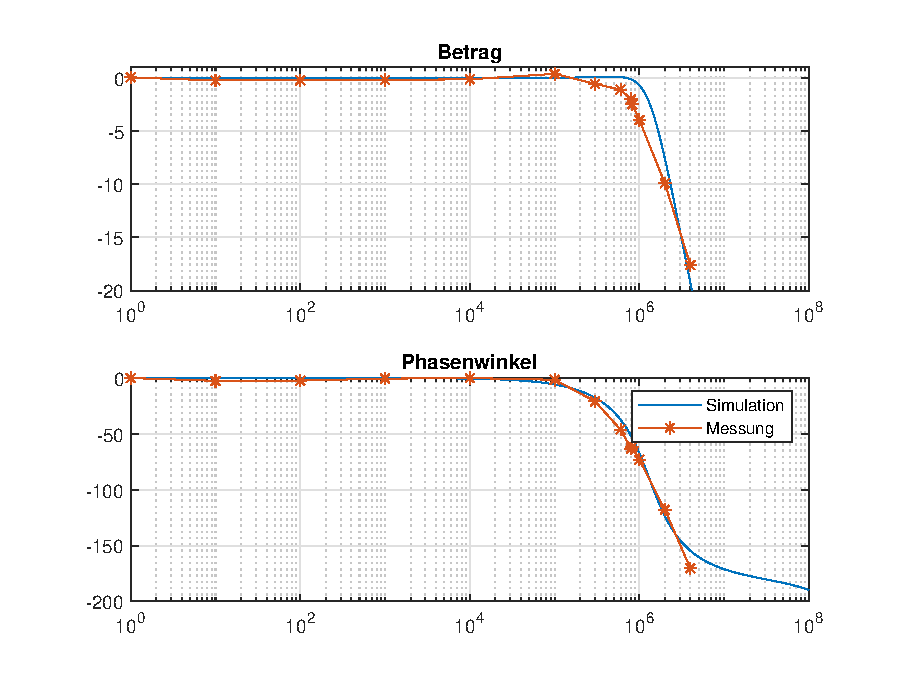
\includegraphics[width=0.8\textwidth]{Lab_1/Plots/Folger.eps}
    \caption{Bodediagramm der Folgerschaltung, $V_{inPP}=100mV$, $V_{CC}=-V_{EE}=15V$}
    \label{fig:Bode_Folger_ua741}
\end{figure}

\begin{table}[H]
\centering
\caption{Aussteuerbereich,  $V_{CC}=-V_{EE}=10V$}
\label{tab:Clip_Folger_ua741}
\begin{tabular}{|l|l|}
\hline
unbelastet       & $R_{Last} = 2k\Omega$ \\ \hline
$V_{CC} - 0,49V$ & $V_{CC} - 1,23V$      \\ \hline
$V_{EE} + 1,67V$ & $V_{EE} + 2,39V$      \\ \hline
\end{tabular}
\end{table}

\begin{figure}[H]
    \centering
    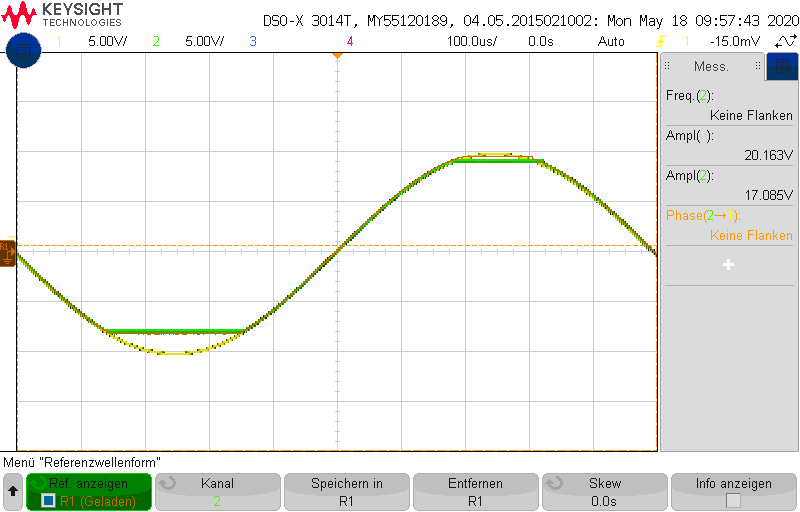
\includegraphics[width=0.8\textwidth]{Lab_1/Messungen/Folger/uberst-schw3.png}
    \caption{Aussteuerbereich $uA741$, $CH_{Ref}: R_{Last} = inf$, $CH_{2}: R_{Last} = 2k\Omega$}
    \label{fig:my_label}
\end{figure}
\begin{figure}[H]
    \centering
    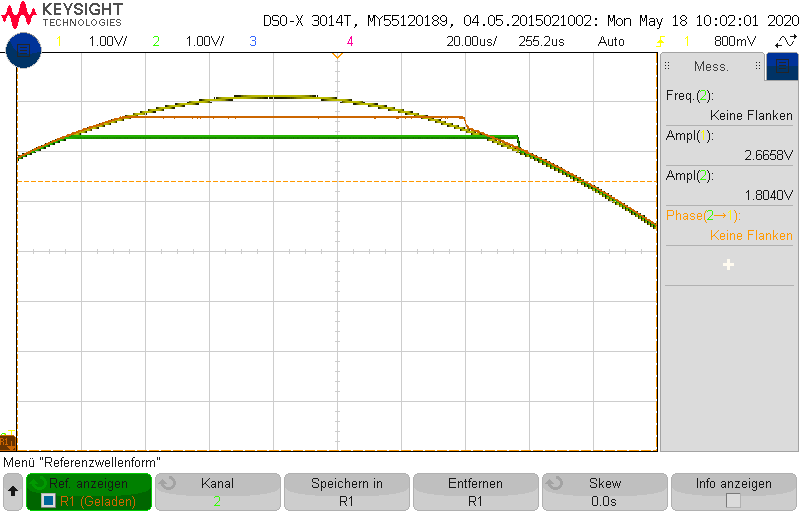
\includegraphics[width=0.8\textwidth]{Lab_1/Messungen/Folger/uberst-schw5.png}
    \caption{Aussteuerbereich Detailansicht $uA741$, $CH_{Ref}: R_{Last} = inf$, $CH_{2}: R_{Last} = 2k\Omega$}
    \label{fig:my_label}
\end{figure}

\begin{figure}[H]
    \centering
    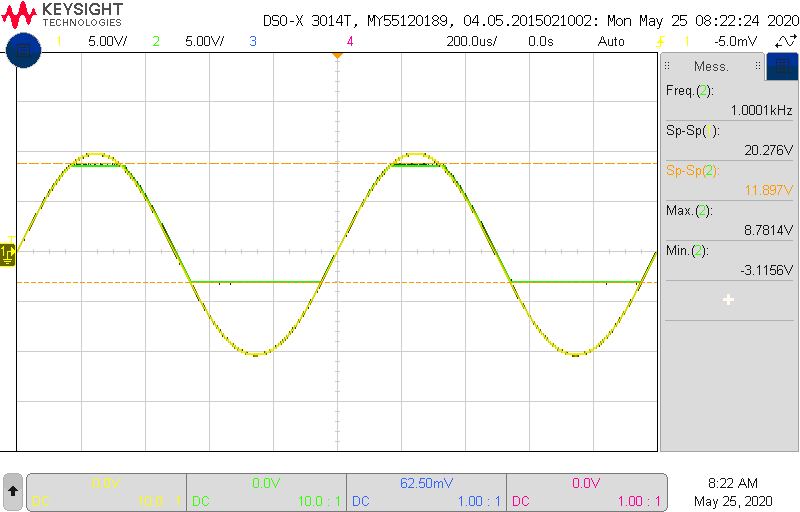
\includegraphics[width=0.8\textwidth]{Lab_1/Messungen/Folger/scope_5.png}
    \caption{Aussteuerbereich $uA741$, $CH_{Ref}: R_{Last} = inf$, $CH_{2}: R_{Last} = 2k\Omega$, $V_{CC} = 10V$, $V_{EE} = -5V$}
    \label{fig:my_label}
\end{figure}

\begin{figure}[H]
    \centering
    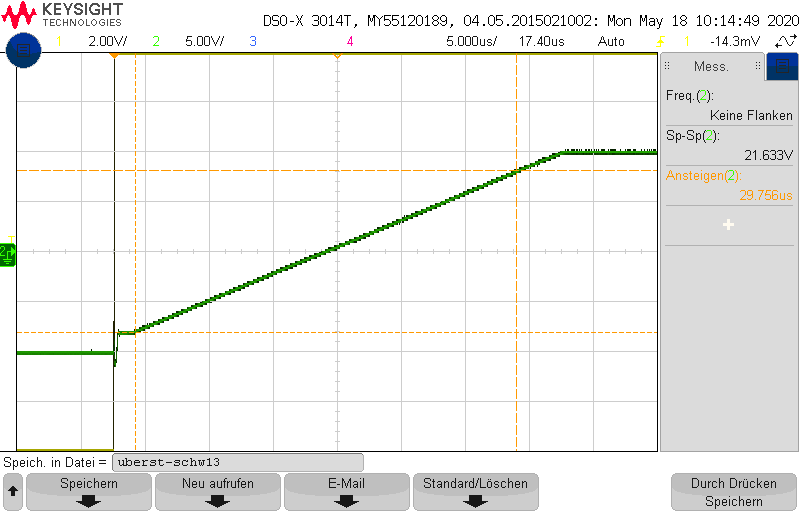
\includegraphics[width=0.8\textwidth]{Lab_1/Messungen/Folger/uberst-schw13.png}
    \caption{Slew Rate $uA741$, $CH_{Ref}$}
    \label{fig:my_label}
\end{figure}

\section{Nicht invertierender Verstärker}
\subsection{Aufgabenstellung}

\begin{figure}[H]
    \centering
    \begin{circuitikz}[]
        \draw (0,0) node[op amp,yscale=-1] (opamp) {\scalebox{1}[-1]{$\mu A 741$}};
        \draw (opamp.down) --++(0,0.5) node[vcc]{$V_{CC}$};
        \draw (opamp.up) --++(0,-0.5) node[vee]{$V_{EE}$};
        
        \draw (opamp.+) to[short,-o] ++(-2,0) node[left] {$U_{in}$};
        \draw (opamp.-) to[short] ++(-0.5,0)
            to[short] ++(0,-2.5)
            to[R=$R_1$] ++(0,-1.5) node[ground]{};
        \draw (opamp.out) to[short,-o] ++(2,0) node[right] {$U_a$};
        \draw (2,0) to[short,*-] ++(0,-2.5)
            to[R=$R_2$,-*] (-1.7,-2.5);
        \end{circuitikz}
    \caption{Nicht invertierender Verstärker}
    \label{fig:niinv_Verst_Schaltung}
 \end{figure}

\subsection{Messaufbau}
\begin{figure}[H]
    \centering
    \begin{circuitikz}[]
        \draw (0,0) node[op amp,yscale=-1] (opamp) {\scalebox{1}[-1]{$\mu A 741$}};
        \draw (opamp.down) --++(0,0.5) node[vcc]{$V_{CC}$};
        \draw (opamp.up) --++(0,-0.5) node[vee]{$V_{EE}$};
        
        \draw (opamp.-) to[short] ++(-0.5,0)
            to[short] ++(0,-2.5)
            to[R=$R_1$] ++(0,-1.5) node[ground]{};
        
        \draw (opamp.out) to[short,-o] ++(3,0)
            %Einfügen der Messchaltung
            to[sV=CH2, color=white, name=S2,o-o] ++(0,-2) node[ground]{};
        \draw (opamp.+) to[short,-o] ++(-2,0) 
            %%Einfügen der Messschaltung
            to[sV=CH1, color=white, name=S1,o-o] ++(0,-2) node[ground] {}
            to[short,o-] ++(-2,0)
            to[sV] ++(0,2)
            to[short,-o] ++(2,0);        
        \draw (2,0) to[short,*-] ++(0,-2.5)
            to[R=$R_2$,-*] (-1.7,-2.5);
            
        \myscope{S1}{0}
        \myscope{S2}{0}

        \end{circuitikz}
    \caption{Nicht invertierender Verstärker, Messaufbau}
    \label{fig:niinv_Verst_Schaltung_Messaufbau}
 \end{figure}


\section{Invertierender Verstärker}
\begin{figure}[H]
    \centering
    \begin{circuitikz}[]
        %%Verstärker und Versorgung
        \draw (0,0) node[op amp] (opamp) {$\mu A 741$};
        \draw (opamp.up) --++(0,0.5) node[vcc]{$V_{CC}$};
        \draw (opamp.down) --++(0,-0.5) node[vee]{$V_{EE}$};
        
        \draw (opamp.+) to[short] ++(-0.25,0)
            to[short] ++(0,-0.25) node[ground] {};
        
        \draw (opamp.-) to[short] (-2,0.5)
            to[R=$R_1$,*-o] ++(-2,0) node[left] {$U_{in}$};
        \draw (-2,0.5) to[short] ++(0,2)
            to[R=$R_2$] ++(4,0)
            to[short,-*] ++(0,-2.5);
        \draw (opamp.out) to[short,-o] ++(2,0) node[right] {$U_a$};
        \end{circuitikz}
    \caption{Invertierender Verstärker}
    \label{fig:inv_verst_Schaltung}
 \end{figure}


\begin{figure}[H]
    \centering
    \begin{circuitikz}[]
        %%Verstärker und Versorgung
        \draw (0,0) node[op amp] (opamp) {$\mu A 741$};
        \draw (opamp.up) --++(0,0.5) node[vcc]{$V_{CC}$};
        \draw (opamp.down) --++(0,-0.5) node[vee]{$V_{EE}$};
        
        \draw (opamp.+) to[short] ++(-0.25,0)
            to[short] ++(0,-0.25) node[ground] {};
        
        \draw (opamp.-) to[short] (-2,0.5)
            to[R=$R_1$,*-o] ++(-2,0)
            %%Einfügen der Messschaltung
            to[sV=CH1, color=white, name=S1,o-o] ++(0,-2) node[ground] {}
            to[short,o-] ++(-2,0)
            to[sV] ++(0,2)
            to[short,-o] ++(2,0);        
        \draw (-2,0.5) to[short] ++(0,2)
            to[R=$R_2$] ++(4,0)
            to[short,-*] ++(0,-2.5);
        \draw (opamp.out) to[short,-o] ++(2,0)        
            %Einfügen der Messchaltung
            to[sV=CH2, color=white, name=S2,o-o] ++(0,-2) node[ground]{};
        \myscope{S1}{0}
        \myscope{S2}{0}
        \end{circuitikz}
    \caption{Invertierender Verstärker, Messaufbau}
    \label{fig:inv_verst_Schaltung_Messaufbau}
 \end{figure}


\section{Addierschaltung}
\begin{figure}[H]
    \centering
    \begin{circuitikz}[]
        %%Verstärker und Versorgung
        \draw (0,0) node[op amp] (opamp) {$\mu A 741$};
        \draw (opamp.up) --++(0,0.5) node[vcc]{$V_{CC}$};
        \draw (opamp.down) --++(0,-0.5) node[vee]{$V_{EE}$};
        
        \draw (opamp.+) to[short] ++(-0.25,0)
            to[short] ++(0,-0.25) node[ground] {};
        
        \draw (opamp.-) to[short] (-2,0.5)
            to[R=$R_1$,*-o] ++(-2,0) node[left] {$U_{in1}$};
        \draw (-2,2.5) to[R=$R_2$,*-o] ++(-2,0) node[left] {$U_{in2}$};
        \draw (-2,0.5) to[short] ++(0,2)
            to[R=$R_{ref}$] ++(4,0)
            to[short,-*] ++(0,-2.5);
        \draw (opamp.out) to[short,-o] ++(2,0) node[right] {$U_a$};
        \end{circuitikz}
    \caption{Addierschaltung}
    \label{fig:Addierschaltung}
 \end{figure}

\begin{figure}[H]
    \centering
    \begin{circuitikz}[]
        %%Verstärker und Versorgung
        \draw (0,0) node[op amp] (opamp) {$\mu A 741$};
        \draw (opamp.up) --++(0,0.5) node[vcc]{$V_{CC}$};
        \draw (opamp.down) --++(0,-0.5) node[vee]{$V_{EE}$};
        
        \draw (opamp.+) to[short] ++(-0.25,0)
            to[short] ++(0,-0.25) node[ground] {};
        
        \draw (opamp.-) to[short] (-2,0.5)
            to[R=$R_1$,*-o] ++(-2,0) to[short] ++(-1,0)             
            %%Einfügen der Messschaltung
            to[sV=CH3, color=white, name=S3,*-*] ++(0,-2) node[ground] {}
            to[short,*-] ++(-2,0)
            to[sV] ++(0,2)
            to[short,-*] ++(2,0);     
        \draw (-2,2.5) to[R=$R_2$,*-o] ++(-2,0) to[short] ++(-4,0)            
        %%Einfügen der Messschaltung
            to[sV=CH1, color=white, name=S1,*-*] ++(0,-2) node[ground] {}
            to[short,*-] ++(-2,0)
            to[sV] ++(0,2)
            to[short,-*] ++(2,0);     ;
        \draw (-2,0.5) to[short] ++(0,2)
            to[R=$R_{ref}$] ++(4,0)
            to[short,-*] ++(0,-2.5);
        \draw (opamp.out) to[short,-o] ++(2,0)            
        to[sV=CH2, color=white, name=S2,o-o] ++(0,-2) node[ground]{};

        \myscope{S1}{0}
        \myscope{S2}{0}
        \myscope{S3}{0}
        \end{circuitikz}
    \caption{Addierschaltung Messaufbau}
    \label{fig:Addierschaltung_Messaufbau}
 \end{figure}


\section{Geräteverzeichnis}
\begin{table}[H]
\centering
\caption{Geräteverzeichnis 1. Übung}
\label{tab:Gerteverzeichnis}
\begin{tabular}{|
>{\columncolor[HTML]{C0C0C0}}l |l|l|l|}
\hline
Gerät           & \cellcolor[HTML]{C0C0C0}Hersteller & \cellcolor[HTML]{C0C0C0}Bezeichnung & \cellcolor[HTML]{C0C0C0}Seriennummer \\ \hline
Multimeter      & Agilent                            & 34450A                              & 9949728                              \\ \hline
Netzteil        & TTI                                & PL303QMD                            & 9949264                              \\ \hline
Signalgenerator & Keysight                           & 33500B Series                       & 9949719                              \\ \hline
Oszilloskop     & Keysight                           & DSO-X 3014T                         & 9949710                              \\ \hline
\end{tabular}
\end{table}

\chapter{Grundschaltungen mit Frequenzgangbeeinflussung}
\section{Spannungsfolger mit LM358}
\subsection{Aufgabenstellung}
Die Schaltung aus Abbildung \ref{fig:Spannungsfolger_LM358_Schaltung} ist auf einem Steckbrett aufzubauen. Danach ist der Verstärker in die negative Versorgungsspannnung zu übersteuern. Dieses Verhalten ist aufzuzeichnen. 
\begin{figure}[H]
    \centering
    \begin{circuitikz}[]
        \draw (0,0) node[op amp] (opamp) {$LM358$};
        \draw (opamp.up) --++(0,0.5) node[vcc]{$V_{CC}$};
        \draw (opamp.down) --++(0,-0.5) node[vee]{$V_{EE}$};
        \draw (opamp.+) to[short,-o] ++(-2,0) node[left] {$U_{In}$};
        \draw (opamp.out) to[short,-o] ++(2,0) node[right] {$U_{a}$};
        \draw (opamp.-) to[short] ++(-1,0)
            to[short] ++(0,2)
            to[short] ++(4,0)
            to[short,-*] ++(0,-2.5);
        \end{circuitikz}
    \caption{Spannungsfolger mit LM358}
    \label{fig:Spannungsfolger_LM358_Schaltung}
 \end{figure}

\subsection{Messaufbau}
Zur Messung der oben genannten Schaltung wurde die Schaltung mit $V_{CC} = 10V$ und $V_{EE} = -7V$ versorgt. Da das Verhalten bei Übersteuerung gezeigt werden sollte und der verwendete Signalgenerator eine maximale $V_{PP} = 20V$ bereitstellen kann, musste hier eine geringere Versorgungspannung als bei vorherigen Messaufbauten verwendet werden
\begin{figure}[H]
    \centering
    \begin{circuitikz}[]
        \draw (0,0) node[op amp] (opamp) {$LM358$};
        \draw (opamp.up) --++(0,0.5) node[vcc]{$V_{CC}$};
        \draw (opamp.down) --++(0,-0.5) node[vee]{$V_{EE}$};
        \draw (opamp.+) to[short,-o] ++(-1,0) 
            %%Einfügen der Messschaltung
            to[sV=CH1, color=white, name=S1,o-o] ++(0,-2) node[ground] {}
            to[short,o-] ++(-2,0)
            to[sV] ++(0,2)
            to[short,-o] ++(2,0);
        \draw (opamp.out) to[short,-o] ++(2,0)
            %Einfügen der Messchaltung
            to[sV=CH2, color=white, name=S2,o-o] ++(0,-2) node[ground]{};
        \draw (opamp.-) to[short] ++(-1,0)
            to[short] ++(0,2)
            to[short] ++(4,0)
            to[short,-*] ++(0,-2.5);
        \myscope{S1}{0}
        \myscope{S2}{0}
        \end{circuitikz}
    \caption{Spannungsfolger mit LM358, Messaufbau zur Bestimmung des zeitlichen Verhaltens}
    \label{fig:Spannungsfolger_LM358_Messaufbau_Offset}
 \end{figure}

\subsection{Interpretation der Messergebnisse}
Der LM358 zeigt bei Aussteurung über den negatigen Gleichtaktaussteuerbereich eine sogenannte Phasenumkehr. Bei der Messung welche in Abbildung \ref{fig:LM358_Phasenumkehr} dargestellt ist, ist gut zu sehen, dass bei Aussteuerung über der Übersteuerung das Signal nicht einfach geklippt wird, sondern eine Phasenumkehr stattfindet. Das heißt konkret, dass in diesem Fall die positive, statt der negativen Versorgungspannung anliegt. 
\begin{figure}[H]
    \centering
    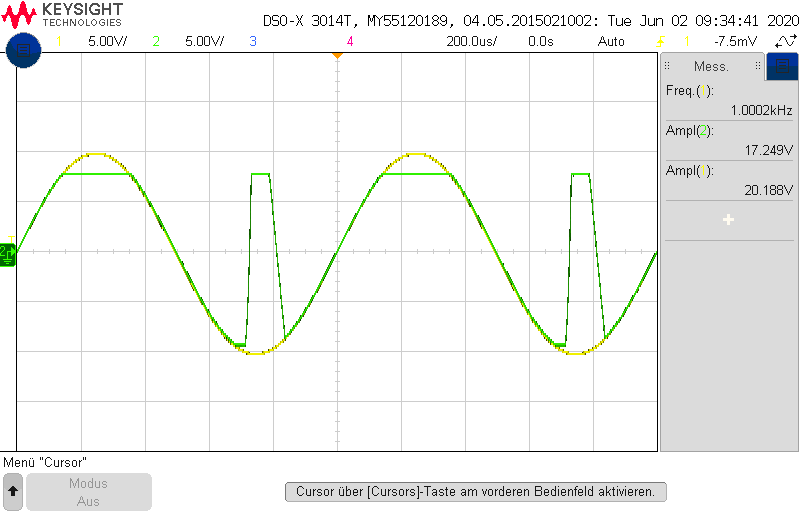
\includegraphics[width = \costumPicWidth]{Lab_2/Messungen/Follower/scope_35.png}
    \caption{LM358 Phasenumkehr bei negativer Übersteuerung}
    \label{fig:LM358_Phasenumkehr}
\end{figure}

%%%%%%%%%%%%%%%%%%%%%%%%%%%%%%%%%%%%%%%%%%%%%%%%%%%%%%%%%%%%%%%%%%%%%%%%%%%%%%%%%%%%%%%%%%%%%%%%%%%%%%%%%%%%%%%%%%%%%%%%%%%%%%
\section{Tiefpass erster Ordnung mit LM358}
\subsection{Aufgabenstellung}
Die in Abbildung \ref{fig:aktiver_Tiefpass_LM358_Schaltung} dargestellte Tiefpassschaltung ist auf eine $f_g=1kHz$ und eine Verstärkung im Durchlassbereich von $\nu = -10$ auszulegen. Die Schaltung ist auf dem Steckbrett aufzubauen.

Danach sind die Grenzfrequenz und die Verstärkung, das Verhalten bei nicht-sinusförmigen Eingangsspannungen und ein Bodediagramm messtechnisch zu erfassen. 
\begin{figure}[H]
    \centering
    \begin{circuitikz}[]
        \draw (0,0) node[op amp] (opamp) {$LM358$};
        \draw (opamp.up) --++(0,0.5) node[vcc]{$V_{CC}$};
        \draw (opamp.down) --++(0,-0.5) node[vee]{$V_{EE}$};
        \draw (opamp.+) to[short] ++(-0.5, 0) to[short] ++(0, -0.5) node[ground]{}; 
        
        \draw (opamp.-) to[R=$R_1$,-o] ++(-2,0) node[left]{$U_{in}$};
        \draw (opamp.-) to[short, *-] ++(0,2)
            to[R=$R_2$,*-*] ++(3,0)
            to[short,-*] ++(0,-2.5)
            to[short] (opamp.out);
        \draw (opamp.-) to[short, *-] ++(0,3.5)
            to[C=$C$] ++(3,0)
            to[short] ++(0,-2);
        \draw (opamp.out) to[short, -o] (3,0) node[right]{$U_{out}$};
        \end{circuitikz}
    \caption{aktiver Tiefpass erster Ordnung}
    \label{fig:Spannungsfolger_LM358_Schaltung}
 \end{figure}

\subsection{Messaufbau}
\begin{figure}[H]
    \centering
    \begin{circuitikz}[]
        \draw (0,0) node[op amp] (opamp) {$LM358$};
        \draw (opamp.up) --++(0,0.5) node[vcc]{$V_{CC}$};
        \draw (opamp.down) --++(0,-0.5) node[vee]{$V_{EE}$};
        \draw (opamp.+) to[short] ++(-0.5, 0) to[short] ++(0, -0.5) node[ground]{}; 
        
        \draw (opamp.-) to[R=$R_1$] ++(-3,0)
            to[sV=CH1, color=white, name=S1,o-o] ++(0,-2) node[ground] {}
            to[short,o-] ++(-2,0)
            to[sV] ++(0,2)
            to[short,-o] ++(2,0);
        \draw (opamp.-) to[short, *-] ++(0,2)
            to[R=$R_2$,*-*] ++(3,0)
            to[short,-*] ++(0,-2.5)
            to[short] (opamp.out);
        \draw (opamp.-) to[short, *-] ++(0,3.5)
            to[C=$C$] ++(3,0)
            to[short] ++(0,-2);
        \draw (opamp.out) to[short, -o] (3,0) 
            to[sV=CH2, color=white, name=S2,o-o] ++(0,-2) node[ground]{};
        
        \myscope{S1}{0}
        \myscope{S2}{0}
        \end{circuitikz}
    \caption{Messaufbau, aktiver Tiefpass erster Ordnung}
    \label{fig:Spannungsfolger_LM358_Schaltung}
 \end{figure}

\subsection{Auslegung der Schaltung}
Bei der Auslegung der Schaltung wurde mit der Berechnung des Widerstandverhältnisses für die Verstärkung begonnen. Danach konnte die Grenzfrequenz der Schaltung mit der Kapazität $C$ bestimmt werden.

\begin{align}
    \nu = -\frac{R_2}{R_1} &= -10\\
    R_1 = 1k\Omega \Rightarrow R_2 &= 10k\Omega\\
    C = \frac{1}{2\pi f_g R_1} &= 15,9nF
\end{align}

\subsection{Interpretation der Messergebnisse}
\begin{figure}[H]
    \centering
    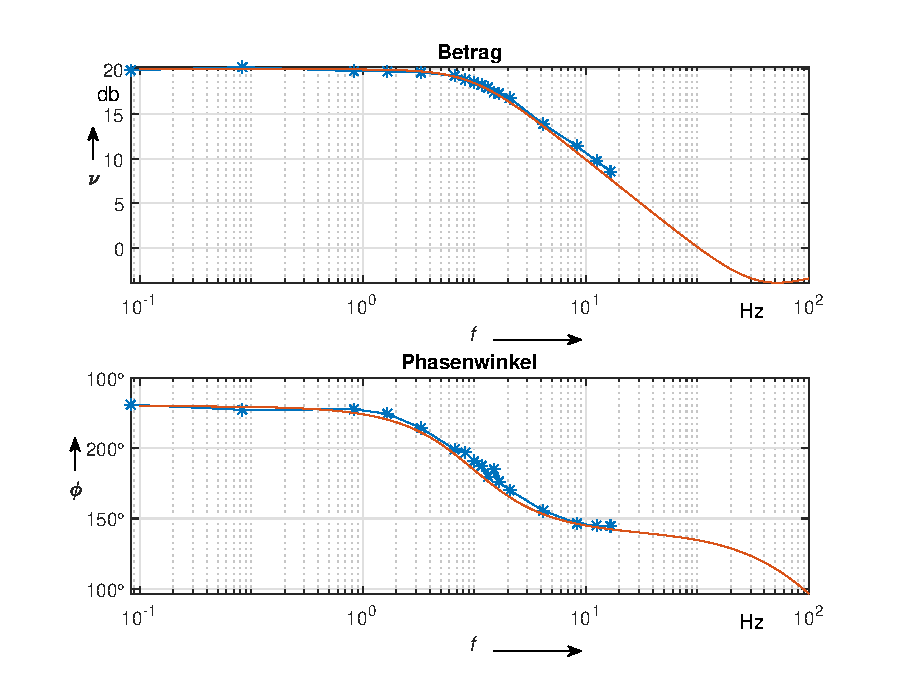
\includegraphics[width=\costumPicWidth]{Lab_2/Plots/TP_first_order.eps}
    \caption{Bodediagramm des Tiefpasses erster Ordnung}
    \label{fig:Bode_aktiver_Tiefpass}
\end{figure}
In diesem Plot ist zu erkennen, dass die Grenzfrequenz bei der Simulation als auch bei den gemessenen Werten bei $f_g = 1kHz$ liegt. 

Der nächste Schritt war der Betrieb der Schaltung mit nicht-sinusförmigen Eingangsspanungen. Konkret wurde hier eine Rechteck und eine Dreieckspannung verwendet.

Um zu verstehen welche Messergebnisse hier zu erwarten sind, sollte an dieser Stelle ein Blick in die Übertragungsfunktion dieser Schaltung gewagt werden.

\begin{align}
    A = -\frac{R_2}{R_1}\frac{1}{1+sR_2 C}
\end{align}
Hier ist an dem Term $\frac{1}{s} $ zu erkennen, dass diese Schaltung integrierendes Verhalten zeigen muss. Durch Kenntnis der unbestimmten Integrale der Eingangsspannungen lassen sich nun Aussagen über die zu erwartenden Ausgangsspannungen treffen.
\subsubsection{Rechteckspannung}
\begin{align}
    \int{1 du} = u + c
\end{align}
Das heißt dass in diesem Fall eine linear ansteigend und abfallende Ausgangsspannung anliegen sollte.

Bei Rechteckspannung die sehr viel kleiner sind als die Grenzfrequenz ist eine Kondensatorladekurve zu sehen, was ebenfalls zu erwarten ist. 

\begin{figure}[H]
    \centering
    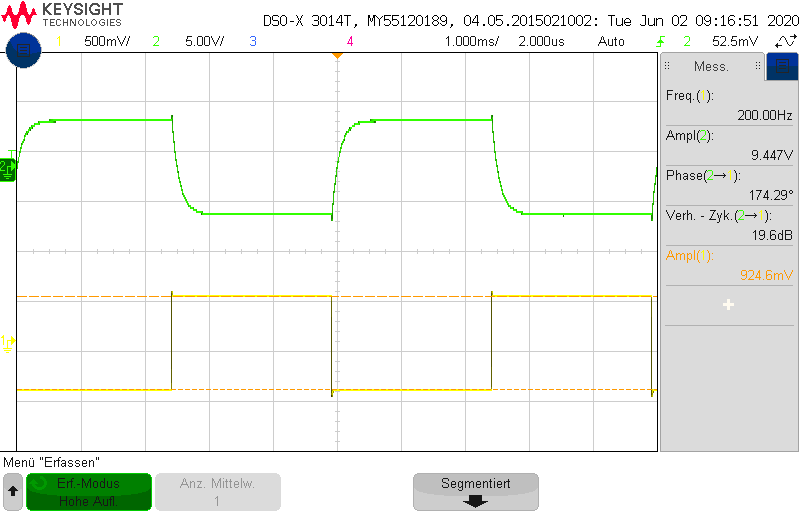
\includegraphics[width=\costumPicWidth]{Lab_2/Messungen/TP_first_order/scope_26.png}
    \caption{Rechteckspannung beim Tiefpass erster Ordnung $f < f_g$}
    \label{fig:Rechteck_Tiefpass_erster_Ordnung_small_f}
\end{figure}
\begin{figure}[H]
    \centering
    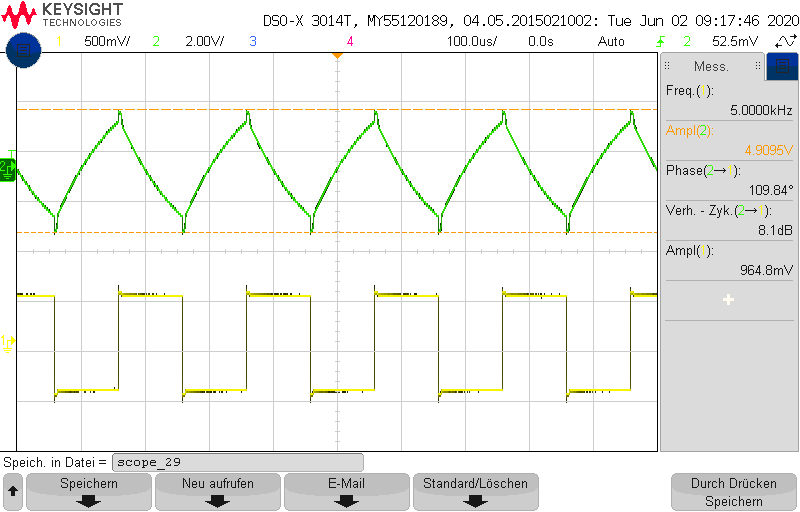
\includegraphics[width=\costumPicWidth]{Lab_2/Messungen/TP_first_order/scope_29.png}
    \caption{Rechteckspannung beim Tiefpass erster Ordnung $f > f_g$}
    \label{fig:Rechteck_Tiefpass_erster_Ordnung_big_f}
\end{figure}

\subsubsection{Dreieckspannung}
Auch in diesem Fall kann die Übertragungsfunktion zu Rate gezogen werden um eine Aussage über die erwartete Ausgangsspannung zu treffen. Bei dieser Eingangsspannung ist lediglich eine anderes unbestimmtes Integral zu lösen.

\begin{align}
    \int{u du} = u^2 + c
\end{align}
Das heißt das nun eine parabelförmige Ausgangsspannung am Ausgang zu erwarten ist.

\begin{figure}[H]
    \centering
    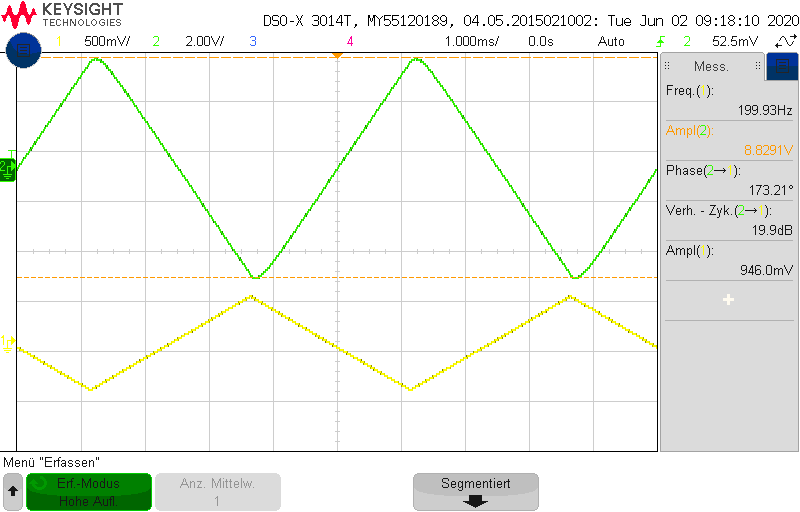
\includegraphics[width=\costumPicWidth]{Lab_2/Messungen/TP_first_order/scope_30.png}
    \caption{Dreieckspannung beim Tiefpass erster Ordnung $f < f_g$}
    \label{fig:Dreieck_Tiefpass_erster_Ordnung_small_f}
\end{figure}
\begin{figure}[H]
    \centering
    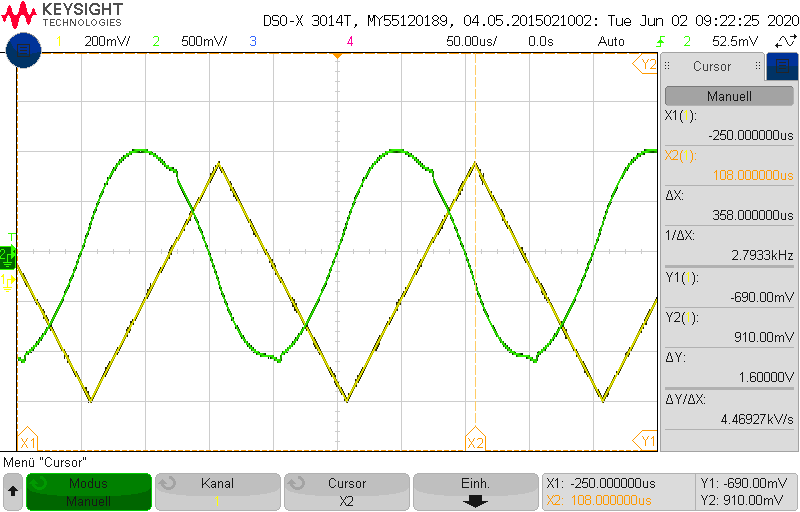
\includegraphics[width=\costumPicWidth]{Lab_2/Messungen/TP_first_order/scope_34.png}
    \caption{Dreieckspannung beim Tiefpass erster Ordnung $f > f_g$}
    \label{fig:Dreieck_Tiefpass_erster_Ordnung_big_f}
\end{figure}
Wie zu erwarten ergab eine dreieckförmige h
\subsection{Ausarbeitungen}

%%%%%%%%%%%%%%%%%%%%%%%%%%%%%%%%%%%%%%%%%%%%%%%%%%%%%%%%%%%%%%%%%%%%%%%%%%%%%%%%%%%%%%%%%%%%%%%%%%%%%%%%%%%%%%%%%%%%%%%%%%%%%%
\section{Hochpass erster Ordnung mit LM358}
\subsection{Aufgabenstellung}
\begin{figure}[H]
    \centering
    \begin{circuitikz}[]
        \draw (0,0) node[op amp] (opamp) {$LM358$};
        \draw (opamp.up) --++(0,0.5) node[vcc]{$V_{CC}$};
        \draw (opamp.down) --++(0,-0.5) node[vee]{$V_{EE}$};
        \draw (opamp.+) to[short] ++(-0.5, 0) to[short] ++(0, -0.5) node[ground]{}; 
        
        \draw (opamp.-) to[R=$R_1$] ++(-2,0) to[C=$C$,-o]++(-2,0) node[left]{$U_{in}$};
        \draw (opamp.-) to[short, *-] ++(0,2)
            to[R=$R_2$] ++(3,0)
            to[short,-*] ++(0,-2.5)
            to[short] (opamp.out);

        \draw (opamp.out) to[short, -o] (3,0) node[right]{$U_{out}$};
        \end{circuitikz}
    \caption{aktiver Hochpass erster Ordnung}
    \label{fig:Hochpass_LM358_Schaltung}
 \end{figure}

\subsection{Messaufbau}
\begin{figure}[H]
    \centering
    \begin{circuitikz}[]
        \draw (0,0) node[op amp] (opamp) {$LM358$};
        \draw (opamp.up) --++(0,0.5) node[vcc]{$V_{CC}$};
        \draw (opamp.down) --++(0,-0.5) node[vee]{$V_{EE}$};
        \draw (opamp.+) to[short] ++(-0.5, 0) to[short] ++(0, -0.5) node[ground]{}; 
        
        \draw (opamp.-) to[R=$R_1$] ++(-2,0) to[C=$C$]++(-2,0) to[short] ++(-1,0)
            to[sV=CH1, color=white, name=S1,o-o] ++(0,-2) node[ground] {}
            to[short,o-] ++(-2,0)
            to[sV] ++(0,2)
            to[short,-o] ++(2,0);
            
        \draw (opamp.-) to[short, *-] ++(0,2)
            to[R=$R_2$] ++(3,0)
            to[short,-*] ++(0,-2.5)
            to[short] (opamp.out);

        \draw (opamp.out) to[short, -o] (3,0) to[sV=CH2, color=white, name=S2,o-o] ++(0,-2) node[ground]{};
        
        \myscope{S1}{0}
        \myscope{S2}{0}
        \end{circuitikz}
    \caption{aktiver Hochpass erster Ordnung}
    \label{fig:Hochpass_LM358_Messaufbau}
 \end{figure}

\subsection{Auslegung der Schaltung}

\subsection{Interpretation der Messergebnisse}

\subsection{Ausarbeitungen}

\chapter{Operationsverstärker - Anwendungen}
\section{Präzisionsgleichrichter mit LM358}
\subsection{Aufgabenstellung}
Die Schaltung aus \autoref{fig:Gleichrichter_Schaltung} ist auf einem Steckbrett aufzubauen, dabei ist das Verhalten mit und ohne dem Kondensator C zu dokumentieren. Außerdem ist der Frequenzbereich zu bestimmen in welchem der Fehler der Schaltung bei unter 1\% bleibt.
\begin{figure}[H]
    \centering
    \begin{circuitikz}[]
        \draw (0,0) node[op amp] (opamp) {$LM358$};
        \draw (opamp.up) --++(0,0.5) node[vcc]{$V_{CC}$};
        \draw (opamp.down) --++(0,-0.5) node[vee]{$V_{EE}$};
        \draw (opamp.+) to[short] ++(-0.5, 0) to[short] ++(0, -0.5) node[ground]{}; 
        
        \draw (opamp.-) to[R=$R$,-o] ++(-3,0) node[left]{$U_{in}$};
        \draw (opamp.-) to[short, *-] ++(0,4) 
            to[R=$R$,-*] ++(3,0) 
            to[D, -*] ++(0,-2) 
            to[D,-*]++(-3,0);
        \draw (opamp.out) to[short] ++(0.616161616161616,0) to[short] ++(0,3);
        \draw (1.5,4.5) to[short] ++(2,0)
            to[sR=$R$, name=sR] ++(0,-3)
            to[short] ++(0,-5)
            to[R=$R$] ++(-7.25,0)
            to[short,-*] ++(0,4);
            
        \draw (sR.label) to[short] ++(0,0.75)
            to[short,-*] ++(0.35,0);
        
        \draw (7,1) node[op amp] (opamp2) {$LM358$};
        \draw (opamp2.up) --++(0,0.5) node[vcc]{$V_{CC}$};
        \draw (opamp2.down) --++(0,-0.5) node[vee]{$V_{EE}$};
        \draw (opamp2.+) to[short] ++(-0.5, 0) to[short] ++(0, -0.5) node[ground]{};         
        
        \draw (opamp2.-) to[short,-*] ++(-2.3,0);
        
        \draw (opamp2.-) to[short, *-] ++(0,2)
            to[R=$R$,*-*] ++(3,0)
            to[short,-*] ++(0,-2.5)
            to[short] (opamp2.out);
        \draw (opamp2.-) to[short, *-] ++(0,3.5)
            to[C=$C$] ++(3,0)
            to[short] ++(0,-2);
        \draw (opamp2.out) to[short, -o] ++(1,0) node[right]{$U_{out}$};
        
        \end{circuitikz}
    \caption{Präzisionsgleichrichter mit LM358}
    \label{fig:Gleichrichter_Schaltung}
 \end{figure}

\subsection{Messaufbau}
Die Schaltung wurde mit dem Signalgenerator betrieben und mit $V_{CC} = -V_{EE} = 15V$ versorgt. Der Ausgang der Schaltung wurde mit dem Oszilloskop erfasst. Bei der Messung des Gleichrichtwertes wurde zusätzlich mit dem Tischmultimeter gemessen.
\subsection{Auslegung der Schaltung}
Alle verwendeten Widerstände wurden mit dem Nominalwert $R=10k\Omega$ ausgelegt. Das hat einerseits den Vorteil, dass die Quelle nur eine sehr geringe Last erfährt und andererseits hatten wir einen $R_{Trim} = 10k\Omega$ Trimmer zur Verfügung. Dieser wurde eingebaut um Bauteiltoleranzen kompensieren zu können und dafür zu sorgen, dass beide Halbwellen des gleichgerichteten Sinus gleich groß sind.

Für die beiden Dioden wurde das Modell 1N4148 verwendet.
\subsection{Interpretation der Messergebnisse}
Wie in Abbildung \ref{fig:sim_Gleichrichter} zu sehen ist, ist für den Aufbau ohne dem Glättungskondesator C ein gleichgerichter Sinus zu erwarten. Für den Aufbau mit C ist eine schwach pulsierende Gleichspannung zu erwarten die dem Gleichrichtwert des Sinus entspricht.
\subsubsection{Gleichrichtwert einer Sinusspannung}
Für die Herleitung dieses Wertes ist die Phasenverschiebung des Eingangssignals irrelevant. Sie wurde deswegen mit $\phi_x = 0$ angenommen. 
\begin{align}
    u(t)_{Signal} =  \hat{u} \cdot \sin(\omega t) \\   
    u_{glr} = \int_{0}{|u(t)_{Signal}|} \\
\end{align}
Da im Falle des gleichgerichteten Sinus das Signal bereits bei $\frac{T}{2}$ periodisch ist gilt:
\begin{align}
x_{glr} = \frac{1}{\frac{T}{2}}\int _{0} ^{\frac{T}{2}} |\hat{x} \cdot \sin{(\omega t)}|dt\\
x_{glr} = \frac{2\hat{x}}{T} \bigl\lbrack -\frac{1}{\omega}\cos{(\omega t)} \bigr\rbrack ^{\frac{T}{2}} _{t=0} \\
x_{glr} = \frac{2}{\pi} \hat{x} = 0,6366\cdot \hat{x}
\end{align}

Das heißt in diesem Fall ist ein Wert der tiefpassgefilterten Spannung von $U_{gr} =\frac{2}{\pi}\cdot U_{pp}$ zu erwarten. Nun wurde die Frequenz erhöht bis eine Abweichung von 1\% von diesem Wert gemessen wurde. Dieser Umstand trat bei einer Frequenz von $f=6,5\kHz$

\begin{figure}[H]
    \centering
    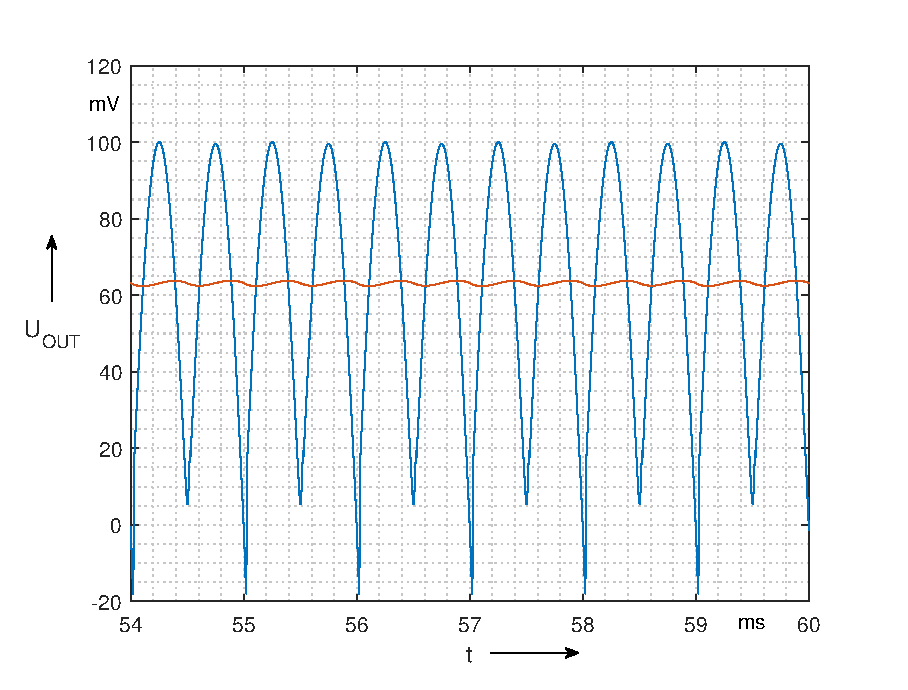
\includegraphics[width=\costumPicWidth]{Lab_3/Plots/Gleichrichter.eps}
    \caption{Simulationsergebnisse des Präzisionsgleichrichters}
    \label{fig:sim_Gleichrichter}
\end{figure}

\begin{figure}[H]
    \centering
    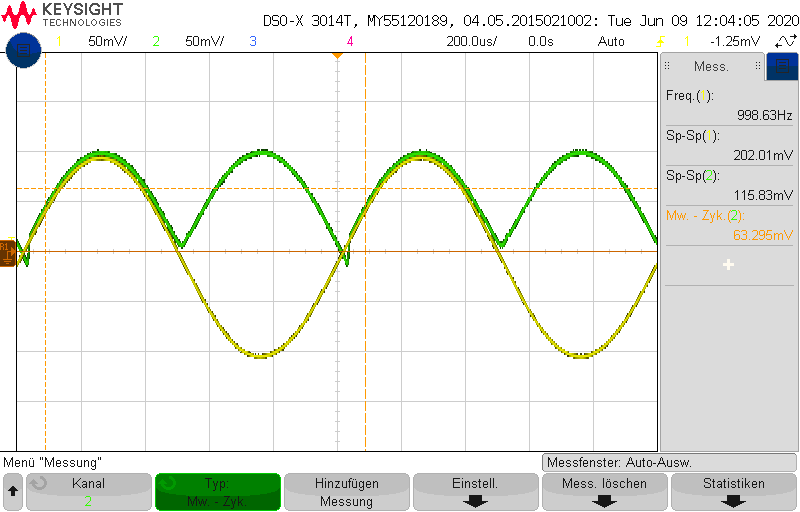
\includegraphics[width=\costumPicWidth]{Lab_3/Messungen/scope_1.png}
    \caption{Gleichrichter ohne C}
    \label{fig:res_gleichrichter_ohne_C}
\end{figure}
\begin{figure}[H]
    \centering
    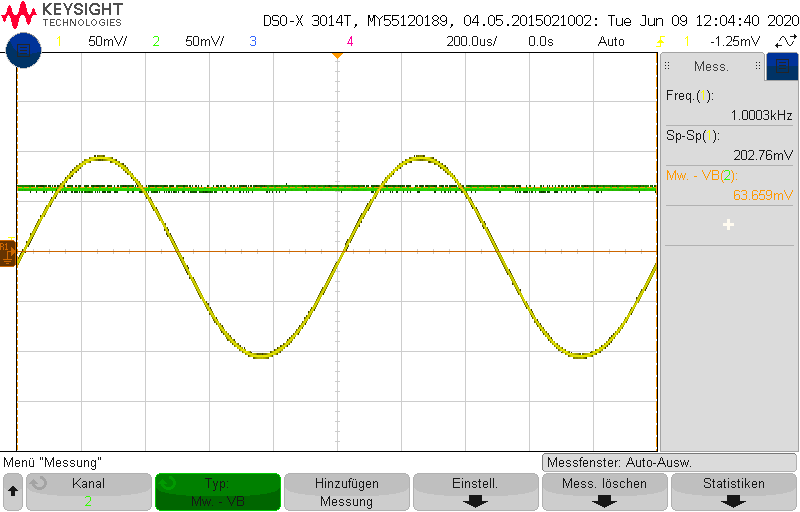
\includegraphics[width=\costumPicWidth]{Lab_3/Messungen/scope_2.png}
    \caption{Gleichrichter mit C}
    \label{fig:res_gleichrichter_mit_C}
\end{figure}
\subsection{Ausarbeitungen}
Ja, für diese Schaltung ist eine Art Offsetabgleich erforderlich. In unserem Fall wurde dies durch den einstellbaren Widerstand $^R/_2$ erreicht worden.

Hier handelt es sich um den arithmetischen Mittelwert. Dieser entspricht dem Gleichrichtwert eines Eingangssignals.
%%%%%%%%%%%%%%%%%%%%%%%%%%%%%%%%%%%%%%%%%%%%%%%%%%%%%%%%%%%%%%%%%%%%%%%%%%%%%%%%%%%%%%%%%%%%%%%

\section{Single Supply Mikrofonverstärker mit LM358 und AD823}
\subsection{Aufgabenstellung}
Die Schaltung aus Abbildung \ref{fig:Mikrofon_Schaltung} soll bei einer Frequenz von $f=30Hz$ eine Verstärkung von $\nu = 40dB$ haben. 
Danach soll die Schaltung auf dem Steckbrett aufgebaut werden und ein Frequenzgang erfasst werden.

Auf einen Versuch mit Mikrofon und Lautsprecher wurde heuer wegen geringerer Laborzeit verzichtet. 

Nach Aufnahme des Amplitudengangs der Schaltung mit dem LM358 wird der Operationsverstärker mit dem pinkompatiblen AD823 ersetzt. Nun wird der Amplitudengang erneut aufgenommen. Diese beiden Amplitudengänge sind zu vergleichen. 
\begin{figure}[H]
    \centering
    \begin{circuitikz}[]
        \draw (0,0) node[op amp,yscale=-1] (opamp) {\scalebox{1}[-1]{$LM358$}};
        \draw (opamp.down) --++(0,0.5) node[vcc]{$V_{CC}$};
        \draw (opamp.up) --++(0,-0.5) node[vee]{$V_{EE}$};

        \draw (opamp.+) to[short] ++(-2,0) to[C=$C_1$,-o] ++(-2,0) node[left]{$U_{in}$};
        \draw (-3,0.5) to[R=$R_5$,*-] ++(0,2) node[vcc]{$V_{CC}$};
        \draw (-3,0.5) to[R=$R_4$,*-] ++(0,-2) node[ground]{};
        
        \draw (opamp.-) to[short] ++(-0.5,0)
            to[short] ++(0,-3)
            to[R=$R_2$] ++(0,-1.5)
            to[C=$C_3$] ++(0,-1.5) node[ground]{};
        \draw (opamp.out) to[short] ++(2,0)
            to[C=$C_2$,-o] ++(1.5,0) node[right]{$U_{out}$};
        \draw (3,0) to[R=$R_3$,*-] ++(0,-2) node[ground]{};
        \draw (2,0) to[short, *-] ++(0,-2.5)
            to[R=$R_1$,-*] ++(-3.7,0);
        \end{circuitikz}
    \caption{Mikrofonverstärker mit LM358 und AD823}
    \label{fig:Mikrofon_Schaltung}
 \end{figure}

\subsection{Messaufbau}
\subsection{Auslegung der Schaltung}
Die Schaltung soll bei $f=30Hz$ bereits eine Verstärkung von $\nu = -100$ aufweisen. Deswegen wurde die Grenzfrequenz der Schaltung mit $f_g=5Hz$ festgelegt. 
Dazu wurden ein paar der Widerstandswerte im Vorhinein angenommen. Mit dem damit resultierenden Tiefpass kann die Kapazität $C_1$ ausgelegt werden.
\begin{align}
    R_4=R_5 &= 100k\Omega \\
    R_{in} = \frac{R_4\cdot R_5}{R_4+ R_5} &= 50k\Omega \\
    C_1=\frac{1}{2\pi f_g R_{in}} = \frac{1}{2\cdot \pi \cdot 5\cdot50\cdot 10^3} &= 636.61nF \approx 2\cdot 330nF = 660nF
\end{align}
Durch die gegebene Verstärkung kann nun der Spannungsteiler $R_1$ und $R_2$ und die Kapazität $C_3$ ausgelegt werden. Die beiden hier verwendeten Widerstände sollten zwar ausreichend groß, jedoch nicht zu groß gewählt werden, da in diesem Bereich der Schaltung parasitäre Kapazitäten sehr leicht zu einem Tiefpassverhalten führen können. Besonders durch den Aufbau auf einem Steckbrett ist diese Schaltung anfällig dafür. 
\begin{align}
    R_1 &= 100k\Omega\\
    \nu = -100 &= -\frac{R_1}{R_2} \\
    R_2 = \frac{R_1}{\nu} &= 1k\Omega\\
    C_3=\frac{1}{2\pi f_g R_2} = \frac{1}{2\cdot \pi \cdot 5\cdot1\cdot 10^3} &= 31,813\mu F \approx 32\mu F
\end{align}
Da die Kapazität $C_2$ lediglich für eine kapazitive Kopplung der Schaltung sorgen soll, wurde ihr Wert willkürlich auf $C_2=100nF$ festgelegt. 

\begin{table}[H]
\centering
\caption{Bauteilwerte Mikrofonverstärker}
\label{tab:Bauteile_Mikrofonv}
\begin{tabular}{|l|r|r|}
\hline
\rowcolor[HTML]{C0C0C0} 
Bauteilname & \multicolumn{1}{l|}{\cellcolor[HTML]{C0C0C0}gewählter Wert} & \multicolumn{1}{l|}{\cellcolor[HTML]{C0C0C0}gemessener Wert} \\ \hline
$R_1$       & $100k\Omega$                                                & $99,491k\Omega$                                              \\ \hline
$R_2$       & $1k\Omega$                                                  & $1,0007k\Omega$                                              \\ \hline
$R_3$       & $100k\Omega$                                                & $98,098k\Omega$                                              \\ \hline
$R_4$       & $100k\Omega$                                                & $99,520k\Omega$                                              \\ \hline
$R_5$       & $100k\Omega$                                                & $98,422k\Omega$                                              \\ \hline
$C_1$       & $660nF$                                                     & $644nF$                                                      \\ \hline
$C_2$       & $100nF$                                                     & $98,5nF$                                                     \\ \hline
$C_3$       & $32\mu F$                                                   & $38,0\mu F$                                                  \\ \hline
\end{tabular}
\end{table}

\subsection{Messergebnisse}
\begin{figure}[H]
    \centering
    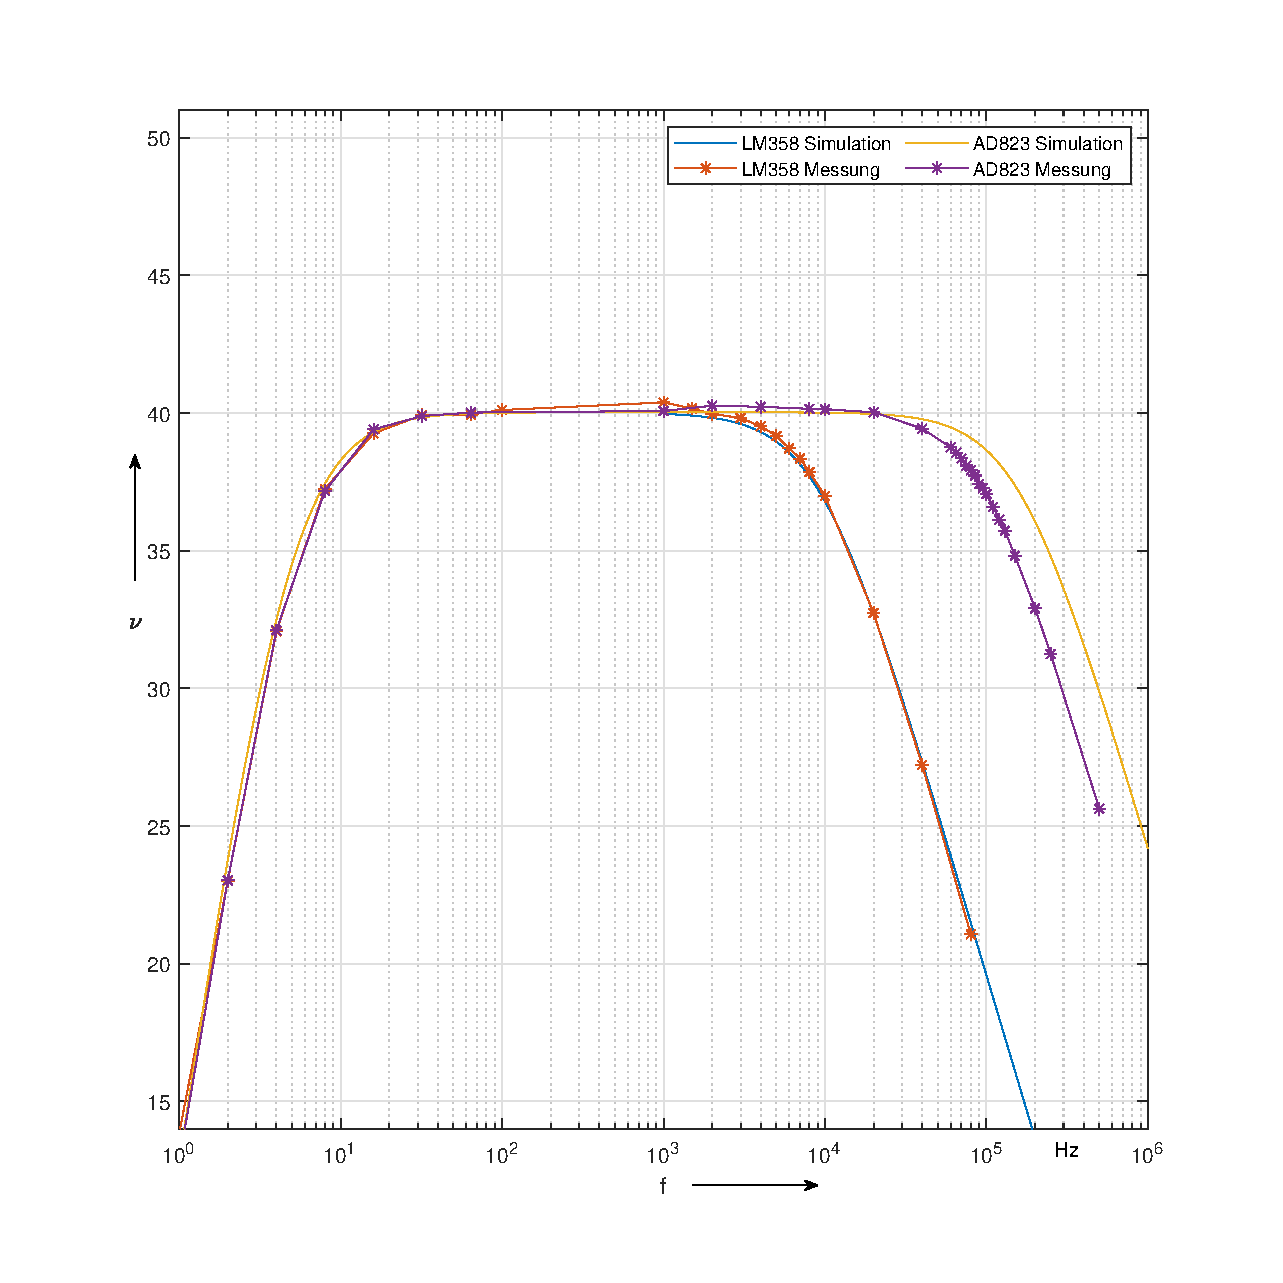
\includegraphics[width=\costumPicWidth]{Lab_3/Plots/Mikrofonverstaerker.eps}
    \caption{Vergleich der Amplitudengänge beim Mikrofonverstärker}
    \label{fig:Amplitudengang_Mikverstaerker}
\end{figure}
\subsection{Interpretation der Messergebnisse} 
Wie in Abbildung \ref{fig:Amplitudengang_Mikverstaerker} zu erkennen ist verhalten sich die real gemessenen Werte, sowie die Schaltungen mit beiden Operationsverstärkern nahezu ident. Die untere Grenzfrequenz liegt bei ungefähr $f_g=8Hz$, das führt dazu, dass bei 30Hz schon nahezu eine Verstärkung von $\nu = 40dB$ erreicht ist.

Bei der oberen Grenzfrequenz ist jedoch nun gut zu erkennen, dass der LM358 das Band bereits sehr viel früher begrenzt, als der AD823. Hier stimmen auch die simulierten Werte mit den gemessenen sehr gut überein. Das liegt vorrangig daran, dass parasitäre Kapauzäten bei solch geringen Frequenzen sehr wenig Einfluss auf die Schaltung haben.

Beim Vergleich der Simulation und der Messung der Schaltung mit dem AD823 ist eine deutlich höhere obere Grenzfrequenz auszumachen. Diese ist bei der gemessenen Schaltung etwas früher, was aber vermutlich an parasitären Kapazitäten im Steckbrett liegt. Dies musste ich während der Laboreinheit erfahren, da der erste Aufbau mit deutlich größeren Widerstandswerten aufgebaut wurde, um die Kapazität $C_3$ möglichst klein zu halten. Dabei erzeugt die Kapazität des Steckbrettes bereits bei $f_g=10^4Hz$ eine obere Grenzfrequenz. 

Für Audioanwendungen ist der AD823 gut geeignet, da der menschliche Hörbereich ungefähr von 16 - 20.000 Hz angegeben wird und die obere Grenzfrequenz bei diesem Verstärker jenseits der 50kHz ist.  Desweiteren beträgt die Samplerate bei MP3 ohnehin nur 44,2kHz, wobei nach dem Abtasttheorem nach Shannon - Nyquist Töne bis maximal 22,1 kHz wiederhergestellt werden können. Der LM358 ist jedenfalls nicht geeignet. Er zeigt bereits bei deutlich zu niedrigen Frequenzen ein Tiefpassverhalten und würde die Qualität des aufgenommenen Signals stark verringern. 
\subsection{Ausarbeitungen}

\section{Sallen-Key Tiefpassfilter}
\subsection{Aufgabenstellung}
Die Schaltung aus Abbildung \ref{fig:Sallen_key} ist auf eine $f_g=30Hz$ und auf eine Verstärkung von $\nu = +10$ auszulegen. Der Filter soll eine Butterworth Charakteristik aufweisen und mit dem Operationsverstärker AD823 auf dem Steckbrett aufgebaut werden.

Von dieser Schaltung ist während der Laboreinheit ein Bodediagramm aufzunehmen und die Sprungantwort zu messen.
\begin{figure}[H]
    \centering
    \begin{circuitikz}[]
        \draw (0,0) node[op amp,yscale=-1] (opamp) {\scalebox{1}[-1]{$AD823$}};
        \draw (opamp.down) --++(0,0.5) node[vcc]{$V_{CC}$};
        \draw (opamp.up) --++(0,-0.5) node[vee]{$V_{EE}$};
        
        \draw (opamp.+) to[short, -*] ++(-2,0)
            to[C=$C_2$] ++(0,-2) node[ground]{};
        \draw (opamp.+) to[short, -*] ++(-2,0)
            to[R=$R_2$] ++(-2,0)
            to[R=$R_1$,-o] ++(-2,0) node[left]{$U_{in}$};
        \draw (-5.25,0.5) to[short,*-] ++(0,2)
            to[C=$C_1$] ++(7.445,0)
            to[short] ++(0,-2.5)
            to[short] (opamp.out);
        \draw (opamp.out) to[short,-*] ++(1,0)
            to[R=$R_4$,-*] ++(0,-3)
            to[R=$R_3$] ++(0,-2) node[ground]{};
        \draw (2.2,-3) to[short] ++(-4,0)
            to[short] ++(0,2.5)
            to[short] (opamp.-);
        \draw (opamp.out) to[short,-o] ++(2,0) node[right] {$U_{out}$};
        \end{circuitikz}
    \caption{Sallen-key, Aktiver Tiefpass}
    \label{fig:Sallen_key}
 \end{figure}


\subsection{Auslegung}
Zur Auslegung dieser Schaltung ist die Übertragungsfunktion \cite[212]{10.5555/3158302} sehr hilfreich.

\begin{align}
    A(s) = \frac{A_0}{1+a_1s + b_1s^2}&=\frac{A_0}{1+\omega_c[C_1(R_1+R_2) + (1-A_0)R_1C_2]s + {\omega_C}^2R_1R_2C_1C_2s^2} \\
    \rm mit \it A_0 &= 1+ \frac{R_4}{R_3} 
\end{align}
Da dieser Filter eine Butterworth Charakteristik aufweisen soll, gilt für $a_1$ und $b_1$:

\begin{align}
    a_1 &= \sqrt{2} \\
    b_1 &= 1
\end{align}

Damit gilt: 
\begin{align}
    a_1 = \sqrt{2} &= \omega_c[C_1(R_1+R_2) + (1-A_0)R_1C_2] \label{eq:a1}\\
    b_1 = 1 &= {\omega_C}^2R_1R_2C_1C_2 \label{eq:b1}
\end{align}

Da im Labor wesentlich weniger verschiedene Kapazitätswerte als Widerstandswerte verfügbar sind, wurde mit der Wahl der Kapazitäten $C_1$ und $C_2$ begonnen. Im Falle der Auslegung einer Schaltung für den realen Einsatz sollte bei der Wahl dieser Kapazitäten auf geringe Toleranzen vom Absolutwert und bei Temperaturdrift wert gelegt werden. Im Labor waren ohnehin nur Kapazitäten mit $\pm10\%$ verfügbar. 

\begin{align}
    C_1 &= 100nF \\
    C_2 &= 330nF
\end{align}

Nach Umformen der Gleichungen \ref{eq:a1} und \ref{eq:b1} ergaben sich folgende Widerstandswerte:

\begin{align}
    R_1 &= 4,28k\Omega \\
    R_2 &= 198,4 k\Omega
\end{align}

\lstinputlisting[language = Matlab, caption=matlab Skript zur Auslegung des aktiven Filter]{Lab_3/auslegung_Sallen_key.m}

\subsection{Simulationsergebnisse}
\begin{figure}[h]
    \centering
    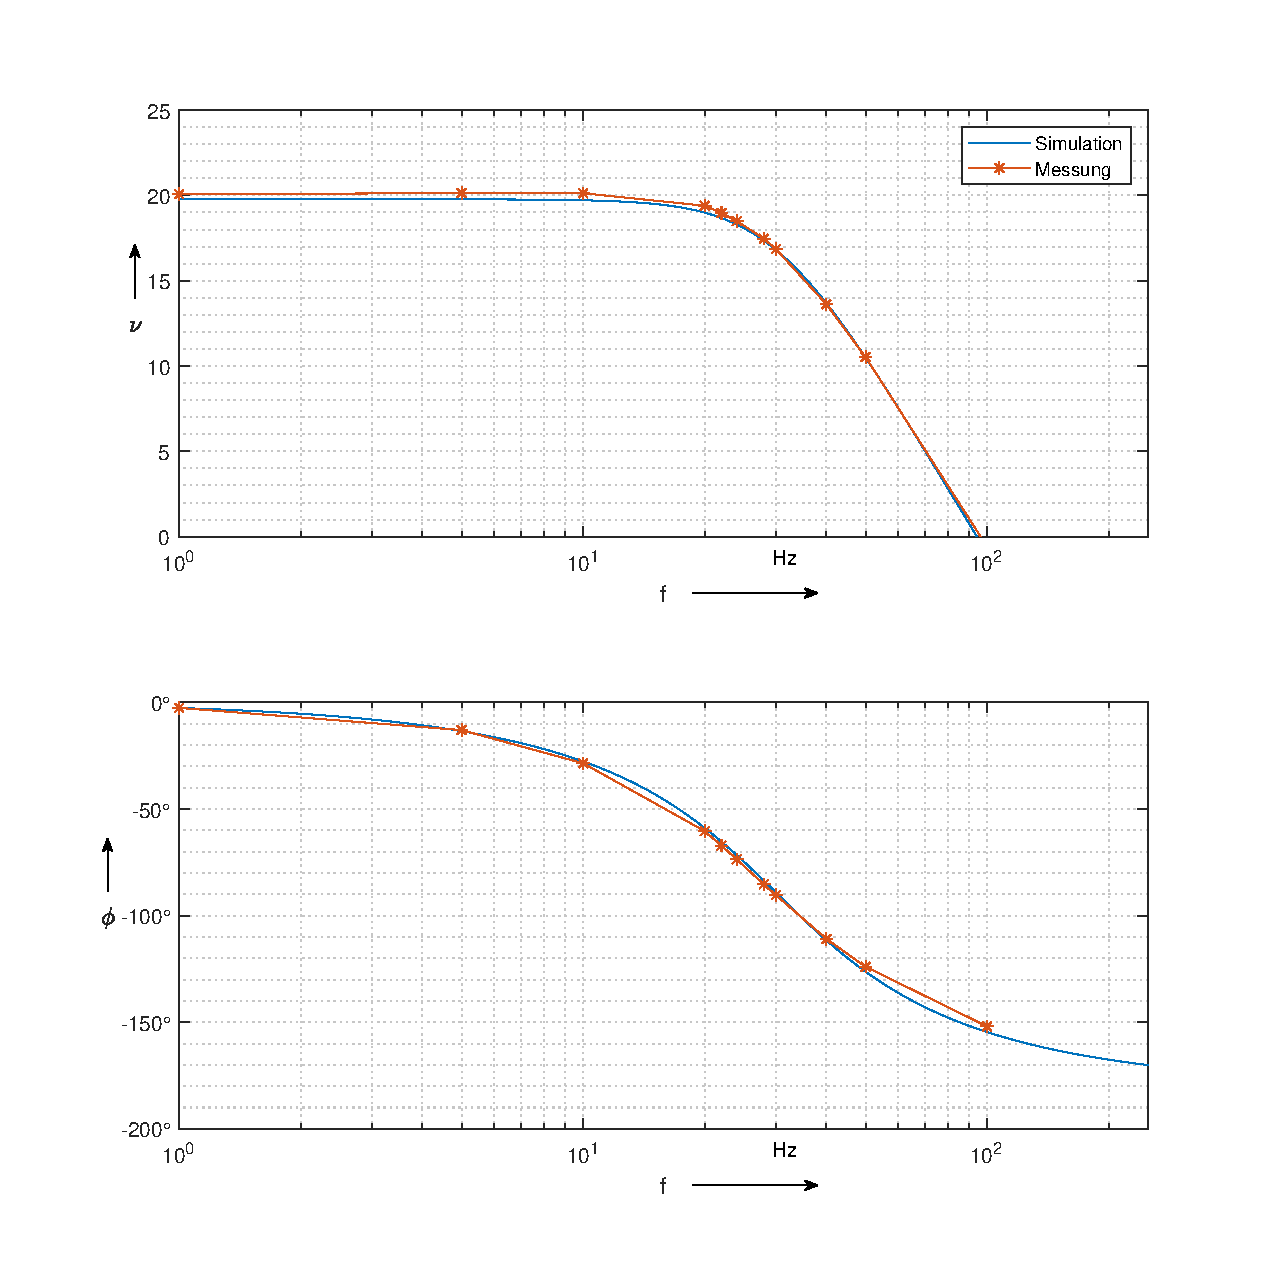
\includegraphics[width = \costumPicWidth]{Lab_3/Plots/sallen_key.eps}
    \caption{Bodediagramm aktiver Tiefpass 2. Ordnung}
    \label{fig:my_label}
\end{figure}

\chapter{Instrumentenverstärker}

testtest
\newpage
\chapter{Signaturen}
    Fertig gestellt am \today \\
    \begin{figure}[H]
        \centering
        
\includegraphics{pics/signature_grebien.png}
    	\caption{Signatur: Grebien Alexander}
    	\label{pic:signatur_grebien}
    \end{figure}
        
\listoffigures
\listoftables
\bibliographystyle{ieeetr}
\bibliography{meine_Zitatsbibliothek.bib}
\end{document}